\documentclass[journal=jacsat,articletitle=true,manuscript=suppinfo,layout=onecolumn]{achemso}

\usepackage{amsmath}
\usepackage{amssymb}
\usepackage{latexsym}
\usepackage{graphicx}
\usepackage{epsfig,epsf,rotating}
\usepackage{url}
\usepackage{subfig}
\usepackage{theorem}
\usepackage{indentfirst}
\usepackage{color}
\usepackage{setspace}
\usepackage{textcomp}
\usepackage{braket}
\usepackage{epstopdf}
\usepackage{mathtools} 
\usepackage{epigraph}
\usepackage{enumitem}
\usepackage{pifont}
\usepackage{xcolor}
\usepackage{graphbox}
\usepackage{booktabs}
\usepackage{multirow}
\usepackage{siunitx}
\usepackage[export]{adjustbox}
\usepackage{tabularx}
\usepackage{pdflscape}
\usepackage[flushleft]{threeparttable}
\usepackage[version=4]{mhchem}

\usepackage{upgreek}
\usepackage{chngpage}
\usepackage{array,booktabs}
\newcolumntype{C}{>{\centering\arraybackslash}X}
\usepackage{nicefrac}
\usepackage{color,soul}
\usepackage{xcolor}
\usepackage{enumitem}
\usepackage{relsize}

\newcommand{\myemph}[1]{\textcolor{red}{\emph{#1}}}


\title{Polarizability Plays a Decisive Role in Modulating Association Between Molecular Cations and Anions}

\author{Chase~E.~Herman}
\affiliation{Department of Chemical and Biomolecular Engineering, 150 Academy St., University of Delaware, Newark, DE 19716, USA}
\author{Arjun~Valiya~Parambathu}
\affiliation{Department of Chemical and Biomolecular Engineering, 150 Academy St., University of Delaware, Newark, DE 19716, USA}
\author{Dilip~N.~Asthagiri}
\affiliation{Oak Ridge National Laboratory, 1 Bethel Valley Rd., Oak Ridge, TN 37830, USA}
\email{asthagiridn@ornl.gov}
\author{Abraham~M.~Lenhoff} %  \corref{cor1}
\affiliation{Department of Chemical and Biomolecular Engineering, 150 Academy St., University of Delaware, Newark, DE 19716, USA}
\email{lenhoff@udel.edu}

\SectionNumbersOn


\begin{document}
\newpage


\tableofcontents

\clearpage

    \section{Unbiased simulations}
    \subsection{Classical molecular dynamics (MD) methods}
    
    Classical molecular dynamics simulations were performed in NAMD (v.\ 2.14 CUDA) \cite{Phillips2020} using the CHARMM36 force field with CMAP corrections (July 2022 release) \cite{Huang2013} along with the CHARMM general force field (CGenFF v.\ 4.6). \cite{Vanommeslaeghe2012} The CHARMM36 \texttt{toppar\_water\_ions.str} file was divided manually into topology and parameter segments to enable its use with \texttt{psfgen} (v.\ 2.0) \cite{Humphrey1996} and NAMD, respectively. Individual \texttt{.sdf} files of polyatomic ions were generated from SMILES strings using the NCI Chemical Identifier Resolver and converted to \texttt{.pdb} files using Open Babel (v.\ 3.1.0). \cite{OBoyle2011} Packmol (v.\ 18.169) \cite{Martinez2009} was used to generate initial coordinates for nine systems, each of which contained one anion species (acetate, ethylsulfonate or methylsulfate) and one cation species (guanidinium, imidazolium or methylammonium). For each system, 22 anion-cation pairs were solvated in 2470 TIP3P\cite{Jorgensen1983} water molecules to form simulation boxes of $\sim$ 42~{\AA} in length, corresponding to a salt concentration of $\sim$ 0.5~M. 
  
    The \texttt{psfgen} utility of VMD (v. 1.9.4a43) \cite{Humphrey1996} was used to generate a \texttt{.psf} structure file for each system, and the partial charges of ion atoms were scaled by a factor of 0.75 for simulations that employed the electronic continuum correction (ECC). \cite{Dijon2020, Leontyev2011, Leontyev2009} All simulations were performed in the $NpT$ ensemble with periodic boundary conditions and parameterized as designed for CGenFF in NAMD (i.e., by reading CHARMM36 protein, carbohydrate, lipid and nucleic acid parameter files prior to CGenFF and water parameters). Time steps of 2~fs were used and the temperature was maintained at 298~K using a Langevin thermostat with a 1~ps$^{-1}$ friction coefficient. A 1~bar pressure was maintained using a Langevin barostat with a 200~fs piston period and a 100~fs decay time and the SHAKE algorithm was used to constrain the geometry of water molecules.\cite{Ryckaert1977} Electrostatic interactions were computed using the particle mesh Ewald (PME) method \cite{Darden1993, Essmann1995} with a grid spacing of 0.5~{\AA} and nonbonded interactions were truncated beyond 9.5~{\AA}. Nonbonded interactions among bonded atoms were treated with a scaled 1-4 exclusion policy without modification of electrostatic interactions between 1-4 atom pairs. A 1~ns equilibration simulation was followed by 100~ns of configurational sampling and frames were saved every 4~ps. 


    \subsection{Semiclassical MD methods}
    Semiclassical simulations were performed in OpenMM (v.\ 7.7.0) \cite{Eastman2017} using the AMOEBA (2018) polarizable force field. \cite{Shi2013} Simulation parameters were generated for ions from \texttt{.sdf} files using Poltype 2 (v.\ 2.3.1) \cite{Walker2022} and appended to the \texttt{amoebabio18.prm} force field file that may be installed with Tinker (v.\ 8.10). \cite{Rackers2018} This was converted to \texttt{.xml} format using OpenMM's  \texttt{processTinkerForceField.py} script without processing ``special pair'' AMOEBA van der Waals parameters, which are not relevant to the systems of interest. A residue entry for each ion was added manually to the resulting \texttt{.xml} file as well as OpenMM's \texttt{residues.xml} file and atom names were assigned according to the CGenFF topology convention. 

    Semiclassical simulations used 1~fs time steps and were performed in mixed precision using the same $NpT$ boundary conditions as classical simulations. The \texttt{LangevinMiddleIntegrator} method was used with a 10~ps$^{-1}$ friction coefficient along with a Monte Carlo barostat. The PME method was used with truncation of nonbonded interactions beyond 10~{\AA} and dipole induction was estimated using the mutual polarization method with a tolerance of $1 \times 10^{-5}$. A 0.2~ns equilibration simulation was followed by 25~ns of configurational sampling and frames were saved every 0.1~ps.


    \subsection{Definition of $R_{Shell}$ for computing $K_A$}
    Potential of mean force (PMF) profiles were computed from simulation trajectories and standard errors of the mean were estimated using the Friedberg-Cameron algorithm.\cite{Friedberg1970, Allen1986} The first local maximum in each PMF profile was identified visually and used as the separation threshold $R_{Shell}$ that delineates whether a given ion pair is in the associated state. Unlike the other PMF profiles, those of imidazolium systems that were simulated using CHARMM36 with the ECC did not exhibit a local maximum following ion-pair contact but they did exhibit an inflection near that separation distance. That point was denoted a ``comparable" $R_{Shell}$ and used to facilitate comparison with the other imidazolium models along with an ``apparent" $R_{Shell}$ value that corresponds to a solvent-separated complex. These values were used to estimate ion-pair association constants $K_{A}$ using Equation~1
    % HARD CODED
    with standard variance addition rules for error propagation. 




    \subsection{Supplementary results from unbiased simulations}
    
    \begin{figure}[H]
    \begin{center}
        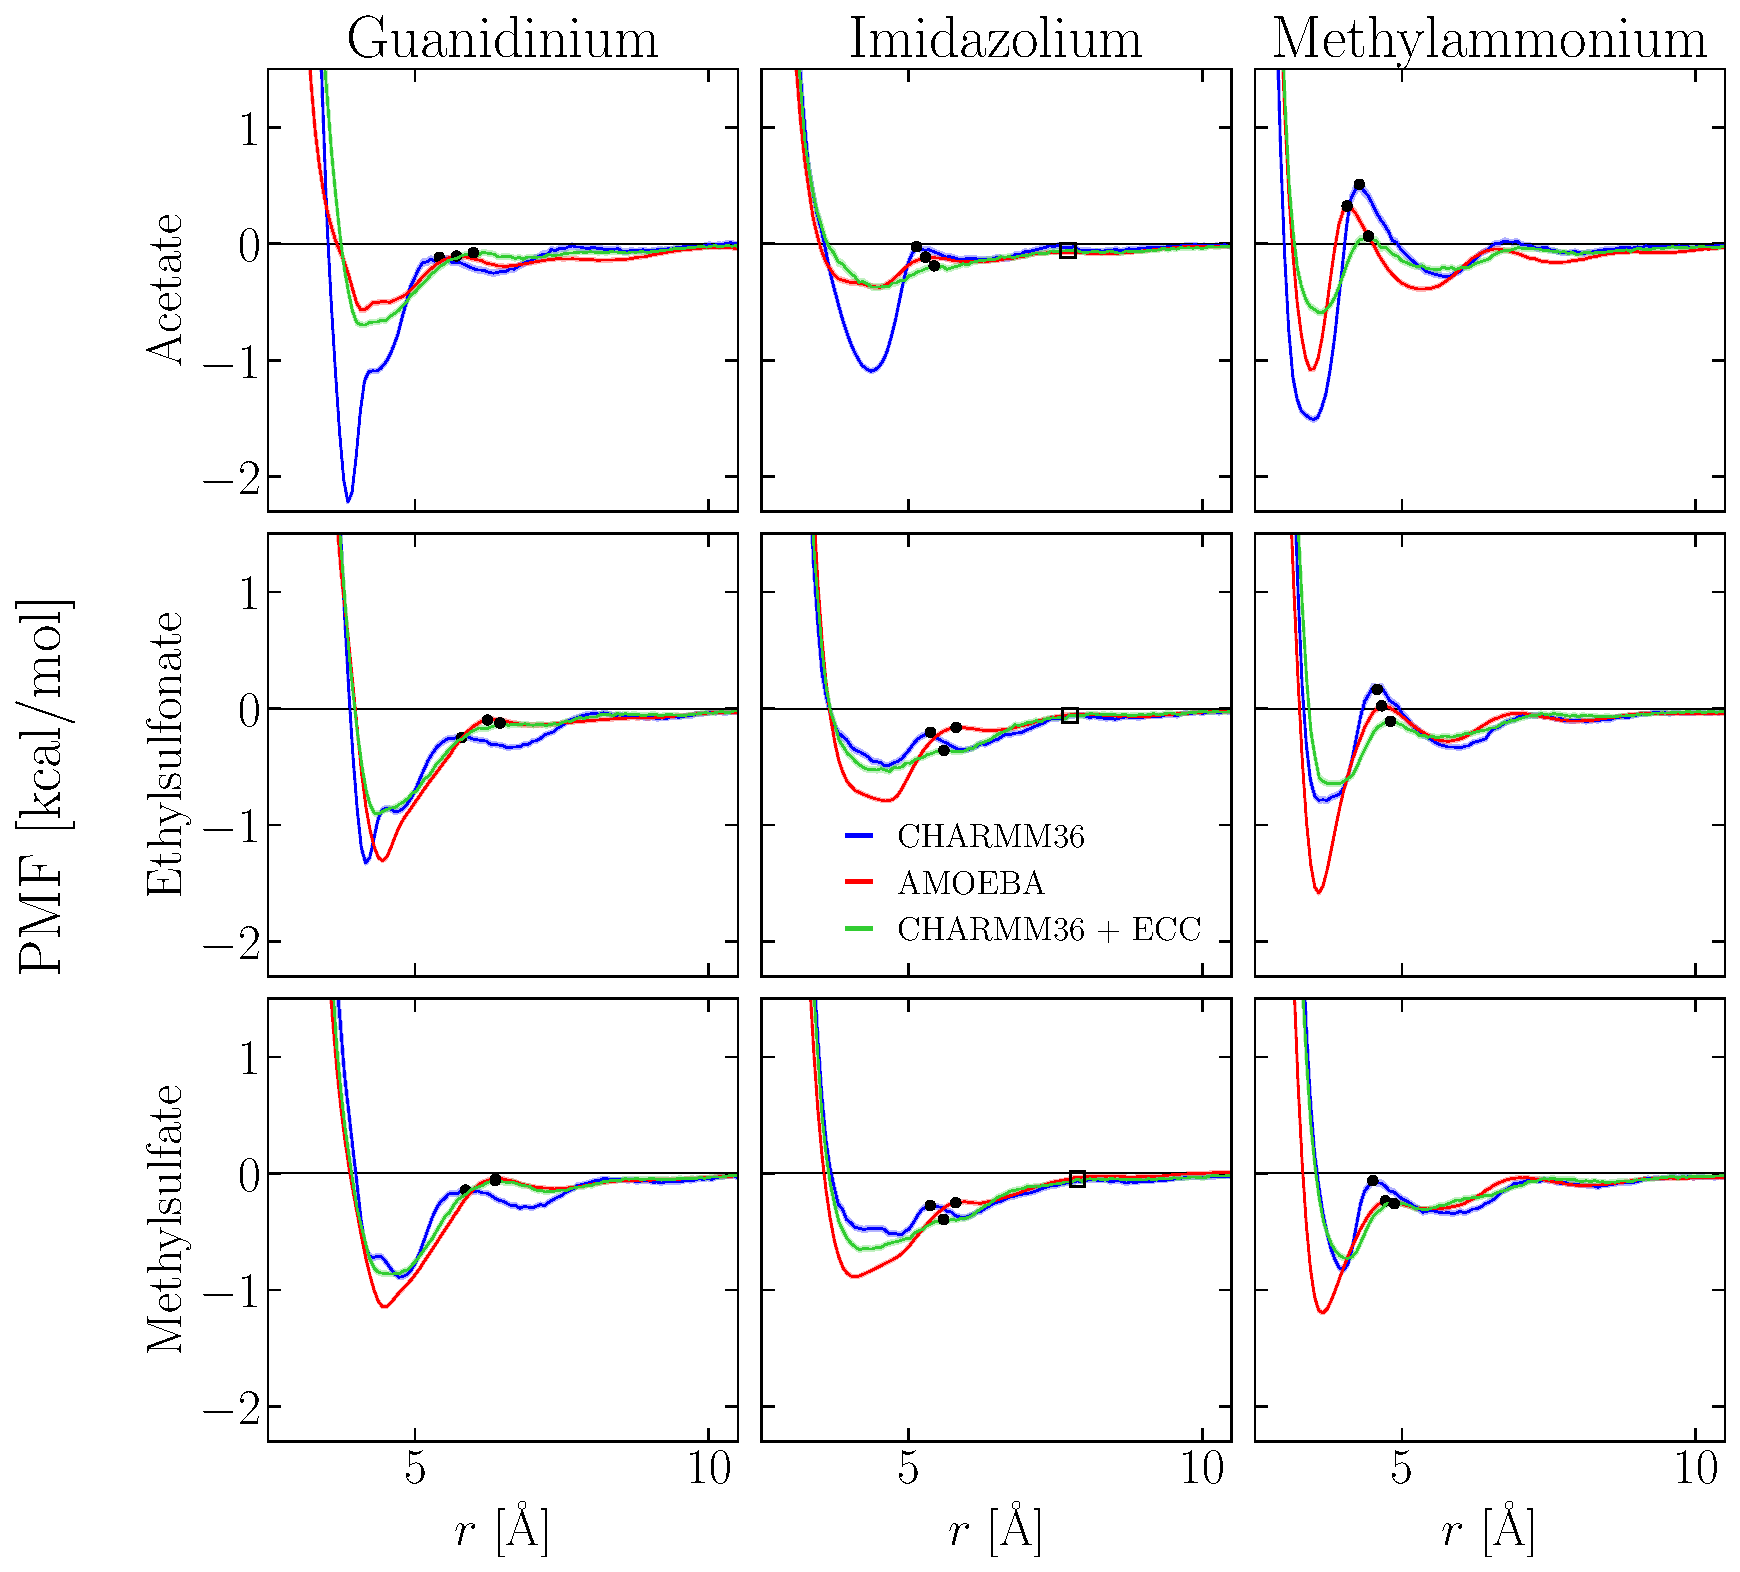
\includegraphics[width=\textwidth]{images/pmfs.pdf}
        \caption{Potential of mean force (PMF) profiles from the interaction of cations (columns) with anions (rows) at a concentration of $\sim$ 0.5 M. The definition of the separation distance $r$ is described in Figure~1 and detailed in Table~\ref{tab:coordinates}. The black points denote the $R_{Shell}$ values that were used for estimating $K_{A}$ in Figure 2
        % HARD CODED
        and represent the comparable $R_{Shell}$ point for the CHARMM36 + ECC imidazolium systems, and black boxes represent the apparent $R_{Shell}$ for those systems. Line widths represent $2\times$ the standard error of the mean.}
        \label{sup-fig:pmfs}
    \end{center}
    \end{figure}

    \begin{figure}[H]
    \begin{center}
        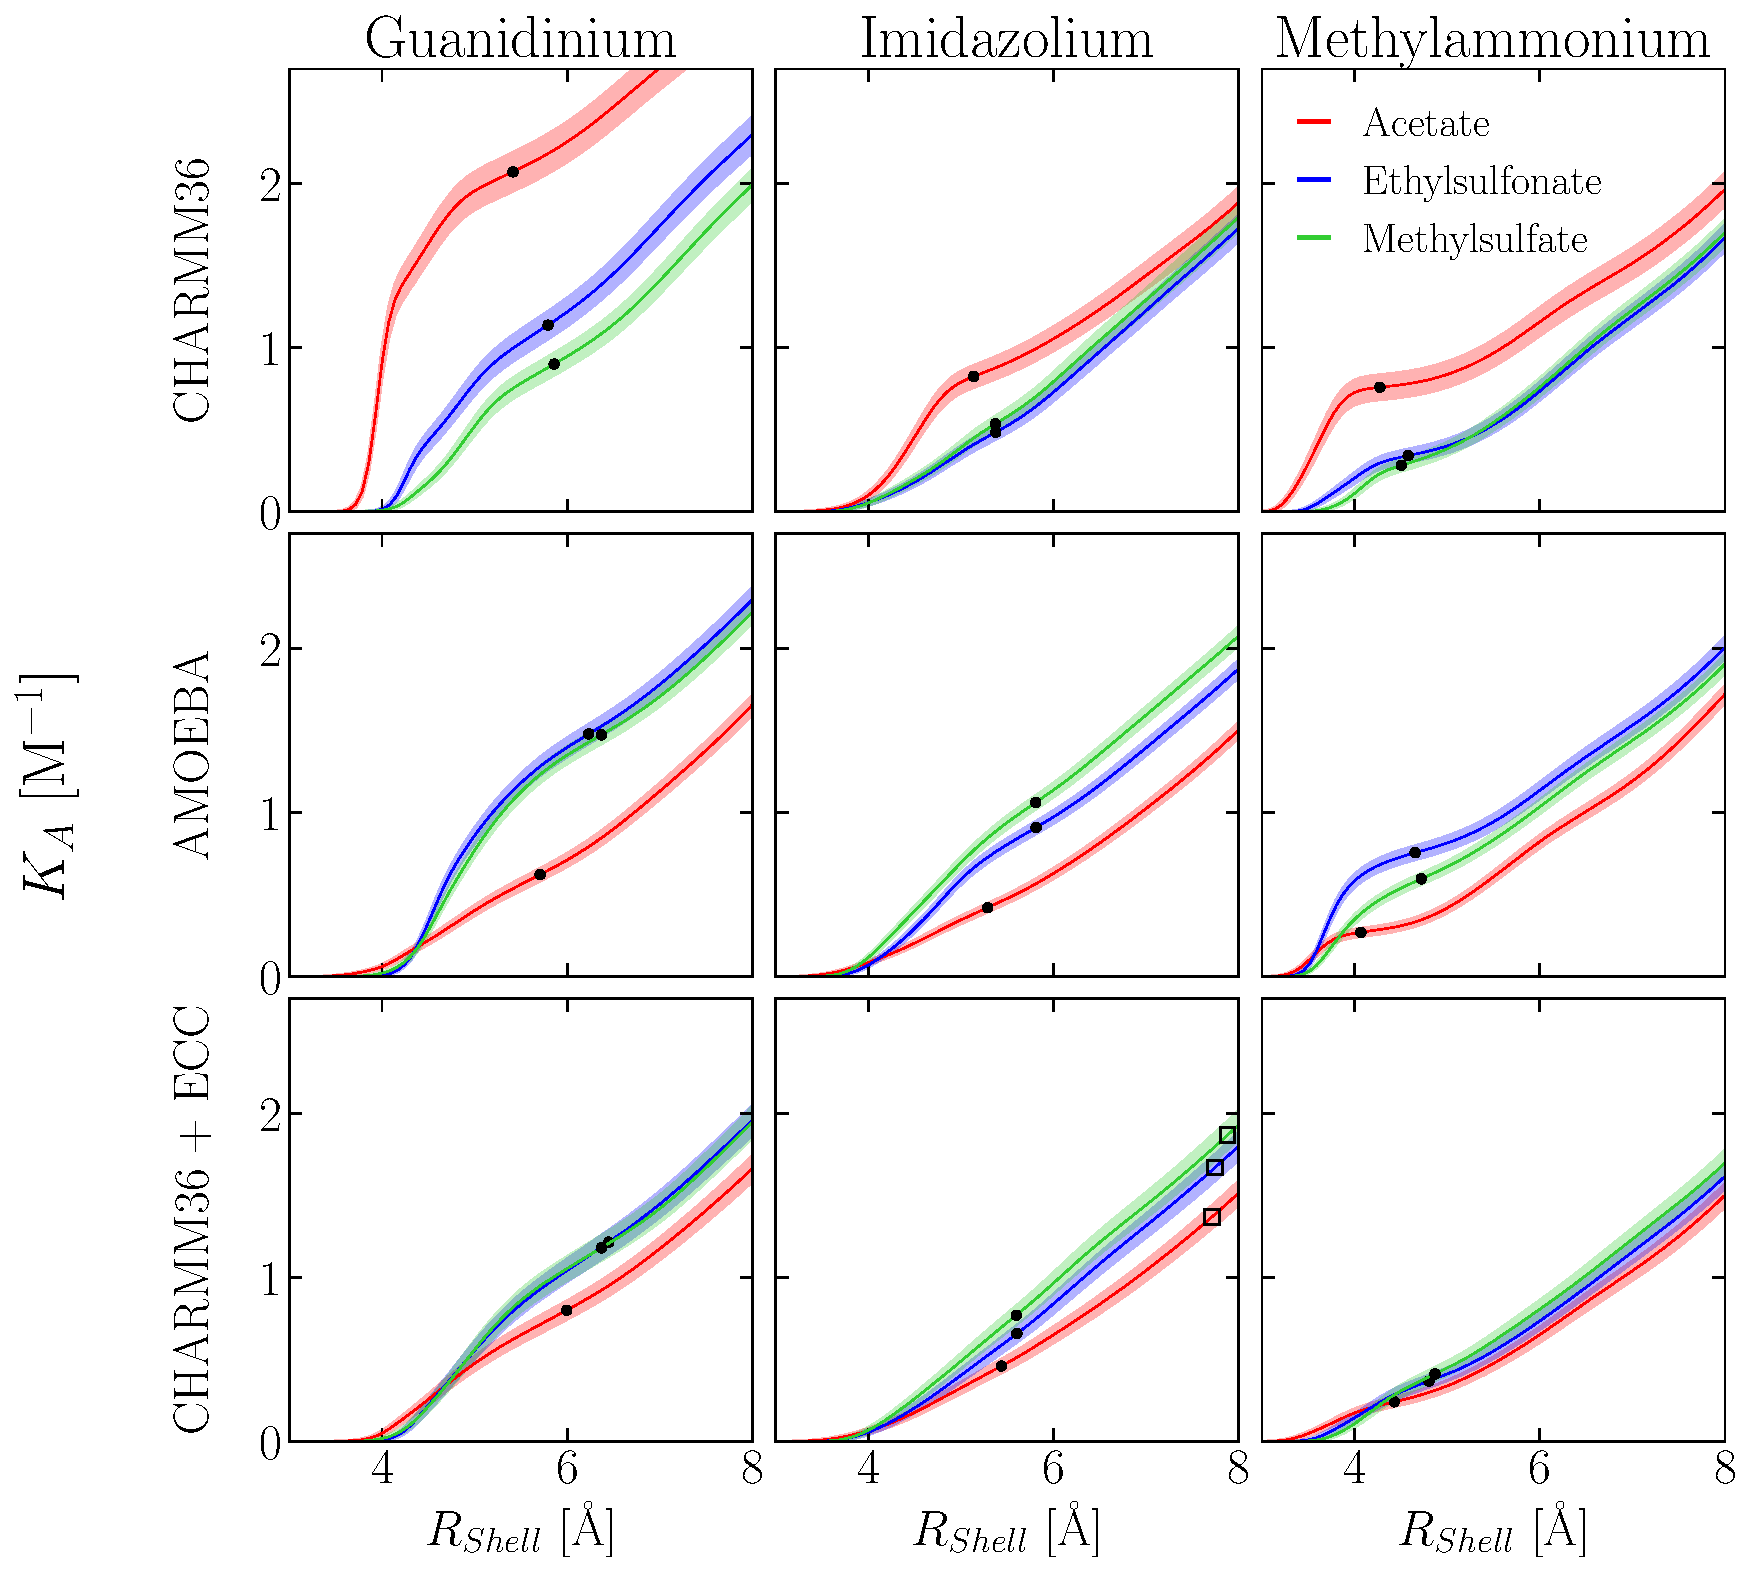
\includegraphics[width=1\columnwidth]{images/Ka_vs_Rshell_anion_comparison.pdf}
        \caption{Dependence of the association constant $K_{A}$ on $R_{Shell}$. Here the rows correspond to the force fields and the lines correspond to the anions. The black points denote the $R_{Shell}$ values that were used for estimating $K_{A}$ in Figure 2
        % HARD CODED
        and represent the comparable $R_{Shell}$ points for the CHARMM36 + ECC imidazolium systems, and black boxes represent the apparent $R_{Shell}$ values for those systems. Shaded regions represent $2\times$ the standard error of the mean.}
        \label{fig:Ka_vs_Rshell}
    \end{center}
    \end{figure}

    
    \begin{adjustbox}{center, caption={$R_{Shell}$, $K_{A}$ and PMF minima of the anion-cation pairs as simulated in the different force fields. Uncertainty values represent the standard error of the mean.}, float=table}
    \label{tab:Ka_data}
    \centering
    \renewcommand{\arraystretch}{0.68}
    \begin{tabular}{l | l | l | c | c | c }
    Force field    & Anion          & Cation          & $R_{Shell}$ [\AA] & $K_{A}$ [M$^{-1}$] & PMF min [kcal/mol] \\
    \hline
    CHARMM36       & Acetate        & Guanidinium     & 5.41  & $2.073 \pm 0.059$ & $-2.215 \pm 0.003$ \\
    CHARMM36       & Ethylsulfonate & Guanidinium     & 5.79  & $1.138 \pm 0.042$ & $-1.321 \pm 0.007$ \\
    CHARMM36       & Methylsulfate  & Guanidinium     & 5.86  & $0.900 \pm 0.034$ & $-0.892 \pm 0.007$ \\
    CHARMM36       & Acetate        & Imidazolium     & 5.14  & $0.825 \pm 0.033$ & $-1.094 \pm 0.006$ \\
    CHARMM36       & Ethylsulfonate & Imidazolium     & 5.38  & $0.485 \pm 0.022$ & $-0.489 \pm 0.008$ \\
    CHARMM36       & Methylsulfate  & Imidazolium     & 5.37  & $0.535 \pm 0.024$ & $-0.530 \pm 0.008$ \\
    CHARMM36       & Acetate        & Methylammonium  & 4.27  & $0.759 \pm 0.038$ & $-1.509 \pm 0.007$ \\
    CHARMM36       & Ethylsulfonate & Methylammonium  & 4.58  & $0.342 \pm 0.020$ & $-0.789 \pm 0.009$ \\
    CHARMM36       & Methylsulfate  & Methylammonium  & 4.51  & $0.283 \pm 0.018$ & $-0.828 \pm 0.008$ \\ \hline
    AMOEBA         & Acetate        & Guanidinium     & 5.71  & $0.622 \pm 0.019$ & $-0.567 \pm 0.008$ \\
    AMOEBA         & Ethylsulfonate & Guanidinium     & 6.23  & $1.479 \pm 0.030$ & $-1.307 \pm 0.004$ \\
    AMOEBA         & Methylsulfate  & Guanidinium     & 6.37  & $1.473 \pm 0.027$ & $-1.147 \pm 0.004$ \\
    AMOEBA         & Acetate        & Imidazolium     & 5.29  & $0.419 \pm 0.013$ & $-0.374 \pm 0.006$ \\
    AMOEBA         & Ethylsulfonate & Imidazolium     & 5.81  & $0.909 \pm 0.019$ & $-0.793 \pm 0.004$ \\
    AMOEBA         & Methylsulfate  & Imidazolium     & 5.81  & $1.061 \pm 0.021$ & $-0.889 \pm 0.004$ \\
    AMOEBA         & Acetate        & Methylammonium  & 4.07  & $0.269 \pm 0.012$ & $-1.077 \pm 0.005$ \\
    AMOEBA         & Ethylsulfonate & Methylammonium  & 4.65  & $0.755 \pm 0.021$ & $-1.585 \pm 0.004$ \\
    AMOEBA         & Methylsulfate  & Methylammonium  & 4.72  & $0.595 \pm 0.017$ & $-1.200 \pm 0.004$ \\ \hline
    CHARMM36 + ECC & Acetate        & Guanidinium     & 5.99  & $0.799 \pm 0.028$ & $-0.698 \pm 0.008$ \\
    CHARMM36 + ECC & Ethylsulfonate & Guanidinium     & 6.45  & $1.215 \pm 0.037$ & $-0.906 \pm 0.007$ \\
    CHARMM36 + ECC & Methylsulfate  & Guanidinium     & 6.37  & $1.179 \pm 0.038$ & $-0.865 \pm 0.007$ \\
    CHARMM36 + ECC & Acetate        & Imidazolium     & 5.44  & $0.459 \pm 0.020$ & $-0.372 \pm 0.009$ \\
    & & (comp. $R_{Shell}$) & & & \\
    CHARMM36 + ECC & Ethylsulfonate & Imidazolium     & 5.60 & $0.656 \pm 0.026$ & $-0.540 \pm 0.007$ \\
    & & (comp. $R_{Shell}$) & & & \\
    CHARMM36 + ECC & Methylsulfate  & Imidazolium     & 5.60 & $0.768 \pm 0.029$ & $-0.658 \pm 0.008$ \\
    & & (comp. $R_{Shell}$) & & & \\
    CHARMM36 + ECC & Acetate        & Imidazolium     & 7.71 & $1.369 \pm 0.035$ & $-0.372 \pm 0.009$ \\
    & & (app. $R_{Shell}$) & & & \\
    CHARMM36 + ECC & Ethylsulfonate & Imidazolium     & 7.75 & $1.671 \pm 0.040$ & $-0.540 \pm 0.007$ \\
    & & (app. $R_{Shell}$) & & & \\
    CHARMM36 + ECC & Methylsulfate  & Imidazolium     & 7.88 & $1.867 \pm 0.043$ & $-0.658 \pm 0.008$ \\
    & & (app. $R_{Shell}$) & & & \\
    CHARMM36 + ECC & Acetate        & Methylammonium  & 4.43  & $0.241 \pm 0.014$ & $-0.590 \pm 0.009$ \\
    CHARMM36 + ECC & Ethylsulfonate & Methylammonium  & 4.80  & $0.367 \pm 0.018$ & $-0.644 \pm 0.008$ \\
    CHARMM36 + ECC & Methylsulfate  & Methylammonium  & 4.87  & $0.410 \pm 0.020$ & $-0.730 \pm 0.008$
    \end{tabular}
    \end{adjustbox}
    \clearpage
    
    \begin{figure}[H]
    \begin{center}
        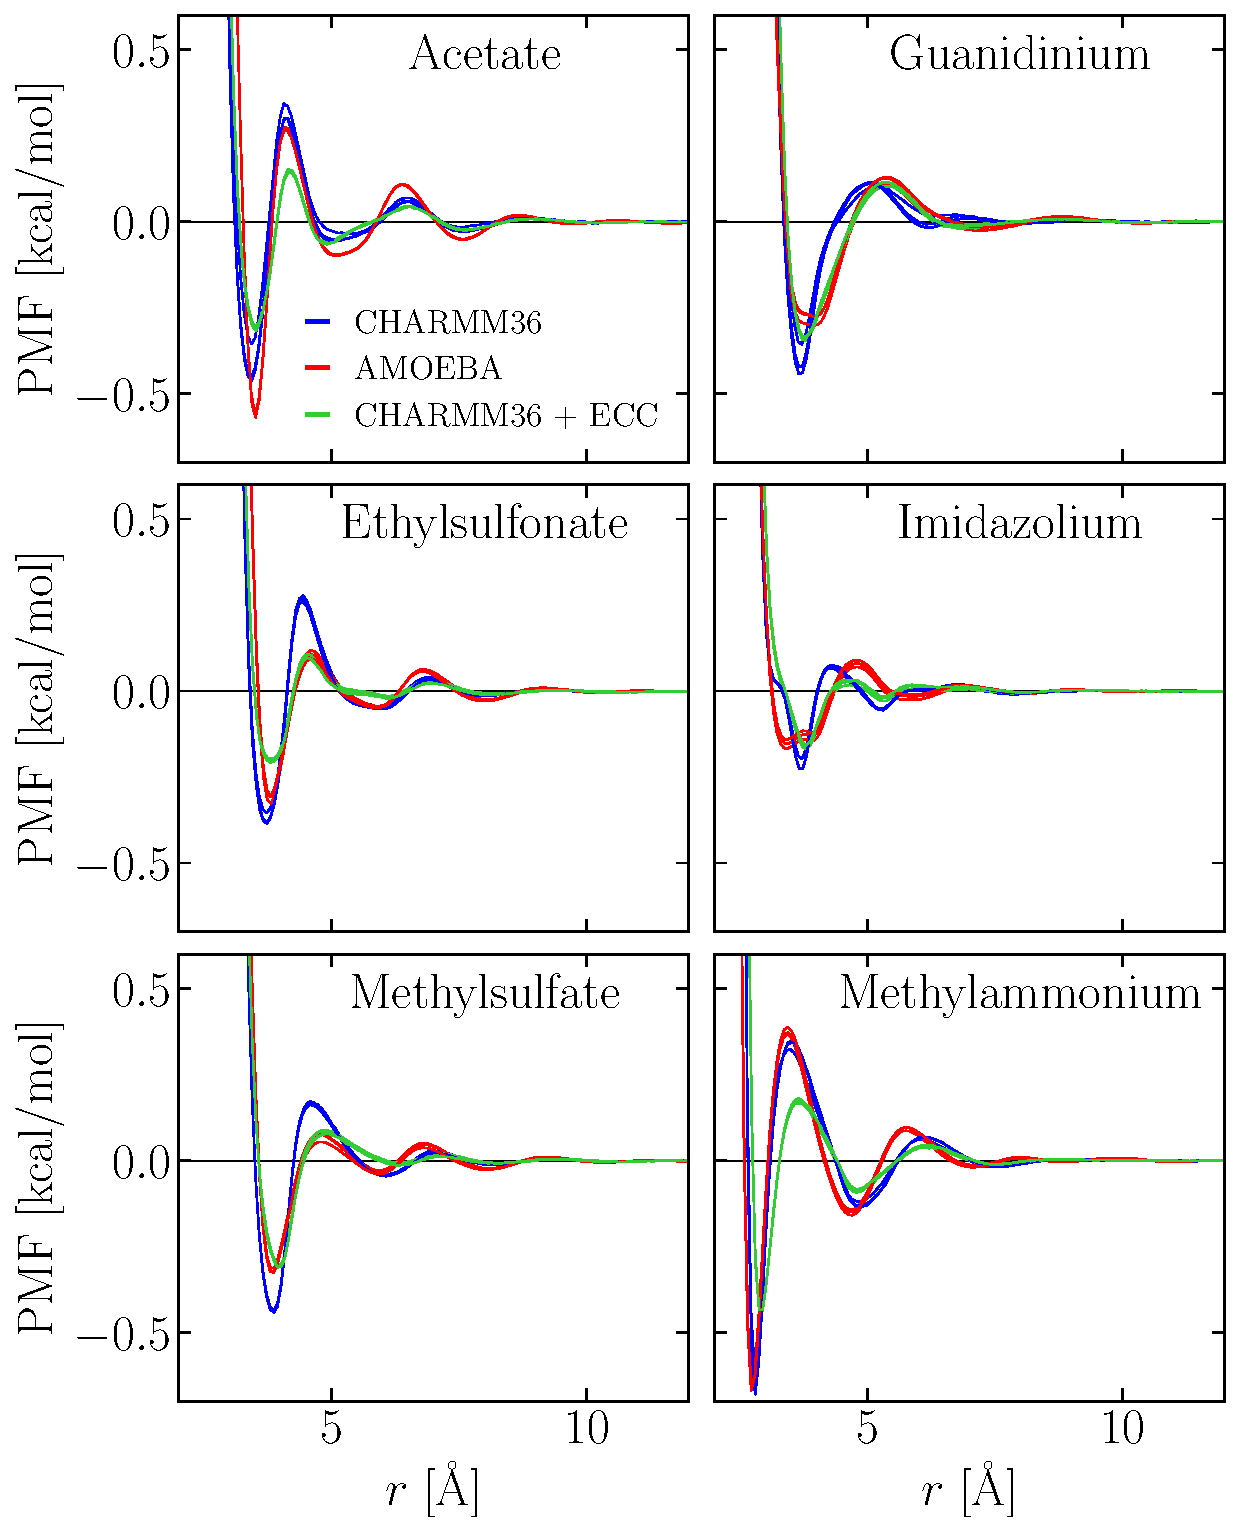
\includegraphics[width=0.9\columnwidth]{images/charmm_comparison_water_overlay_pmf.pdf}
        \caption{Overlay of ion-water potential of mean force (PMF) profiles from simulations with the three counterions, where $r$ is defined in this plot as the separation distance between the water oxygen atom and the ``central" ion atom that is highlighted in Figure 1 with a grey or blue circle (for anions and cations, respectively).}
        \label{fig:water_pmfs}
    \end{center}
    \end{figure}

    \begin{figure}[H]
    \begin{center}
        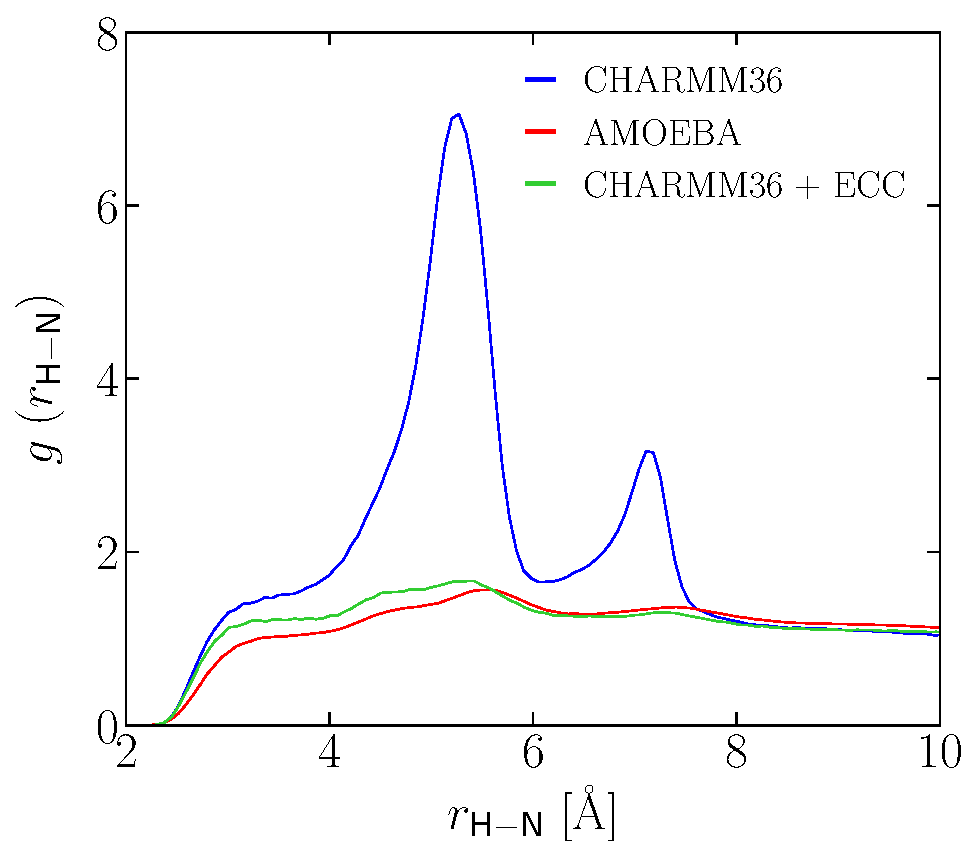
\includegraphics[width=0.6\columnwidth]{images/acet_H_guan_N_gr.pdf}
        \caption{Radial distribution function between acetate hydrogen and guanidinium nitrogen atoms (separation distance $r_{\rm{H-N}}$) for comparison with Mason et al.\cite{Mason2019a}}
        \label{fig:gr_out_of_plane}
    \end{center}
    \end{figure}




    % \clearpage
    \section{\emph{In vacuo} energy analyses}
    
    \subsection{Methods}
    To estimate the underlying balance of attractive and repulsive forces that manifest as ion-pair association, the \emph{in vacuo} interaction energy between every anion-cation pair was computed for all configurations in the simulation trajectories. The \texttt{pairInteraction} module in NAMD was used to analyze both the CHARMM36 and AMOEBA trajectories using the CHARMM36 force field and electrostatic contributions were computed directly (i.e., without PME) with truncation at half the box length to obviate the need for Ewald self-interaction corrections. To enable a comparable analysis of the AMOEBA trajectories with the AMOEBA force field, \texttt{.arc} files of individual ions and anion-cation pairs were generated and used as input to the Tinker potential energy program \texttt{analyze}, with the potential energies of individual ions subtracted from the respective ion pairs. The contributions to the total \emph{in vacuo} interaction energy $U_{Total}$ of ion pairs were then binned according to the separation distance $r$ and ensemble-averaged. The solvent opposition to ion-pair association was inferred as $W_{Solv}~=~w~-~U_{Total}$, where $w$ represents the PMF.



    \subsection{Cross-FF analysis results}
    
    \begin{figure}[H]
    \begin{center}
        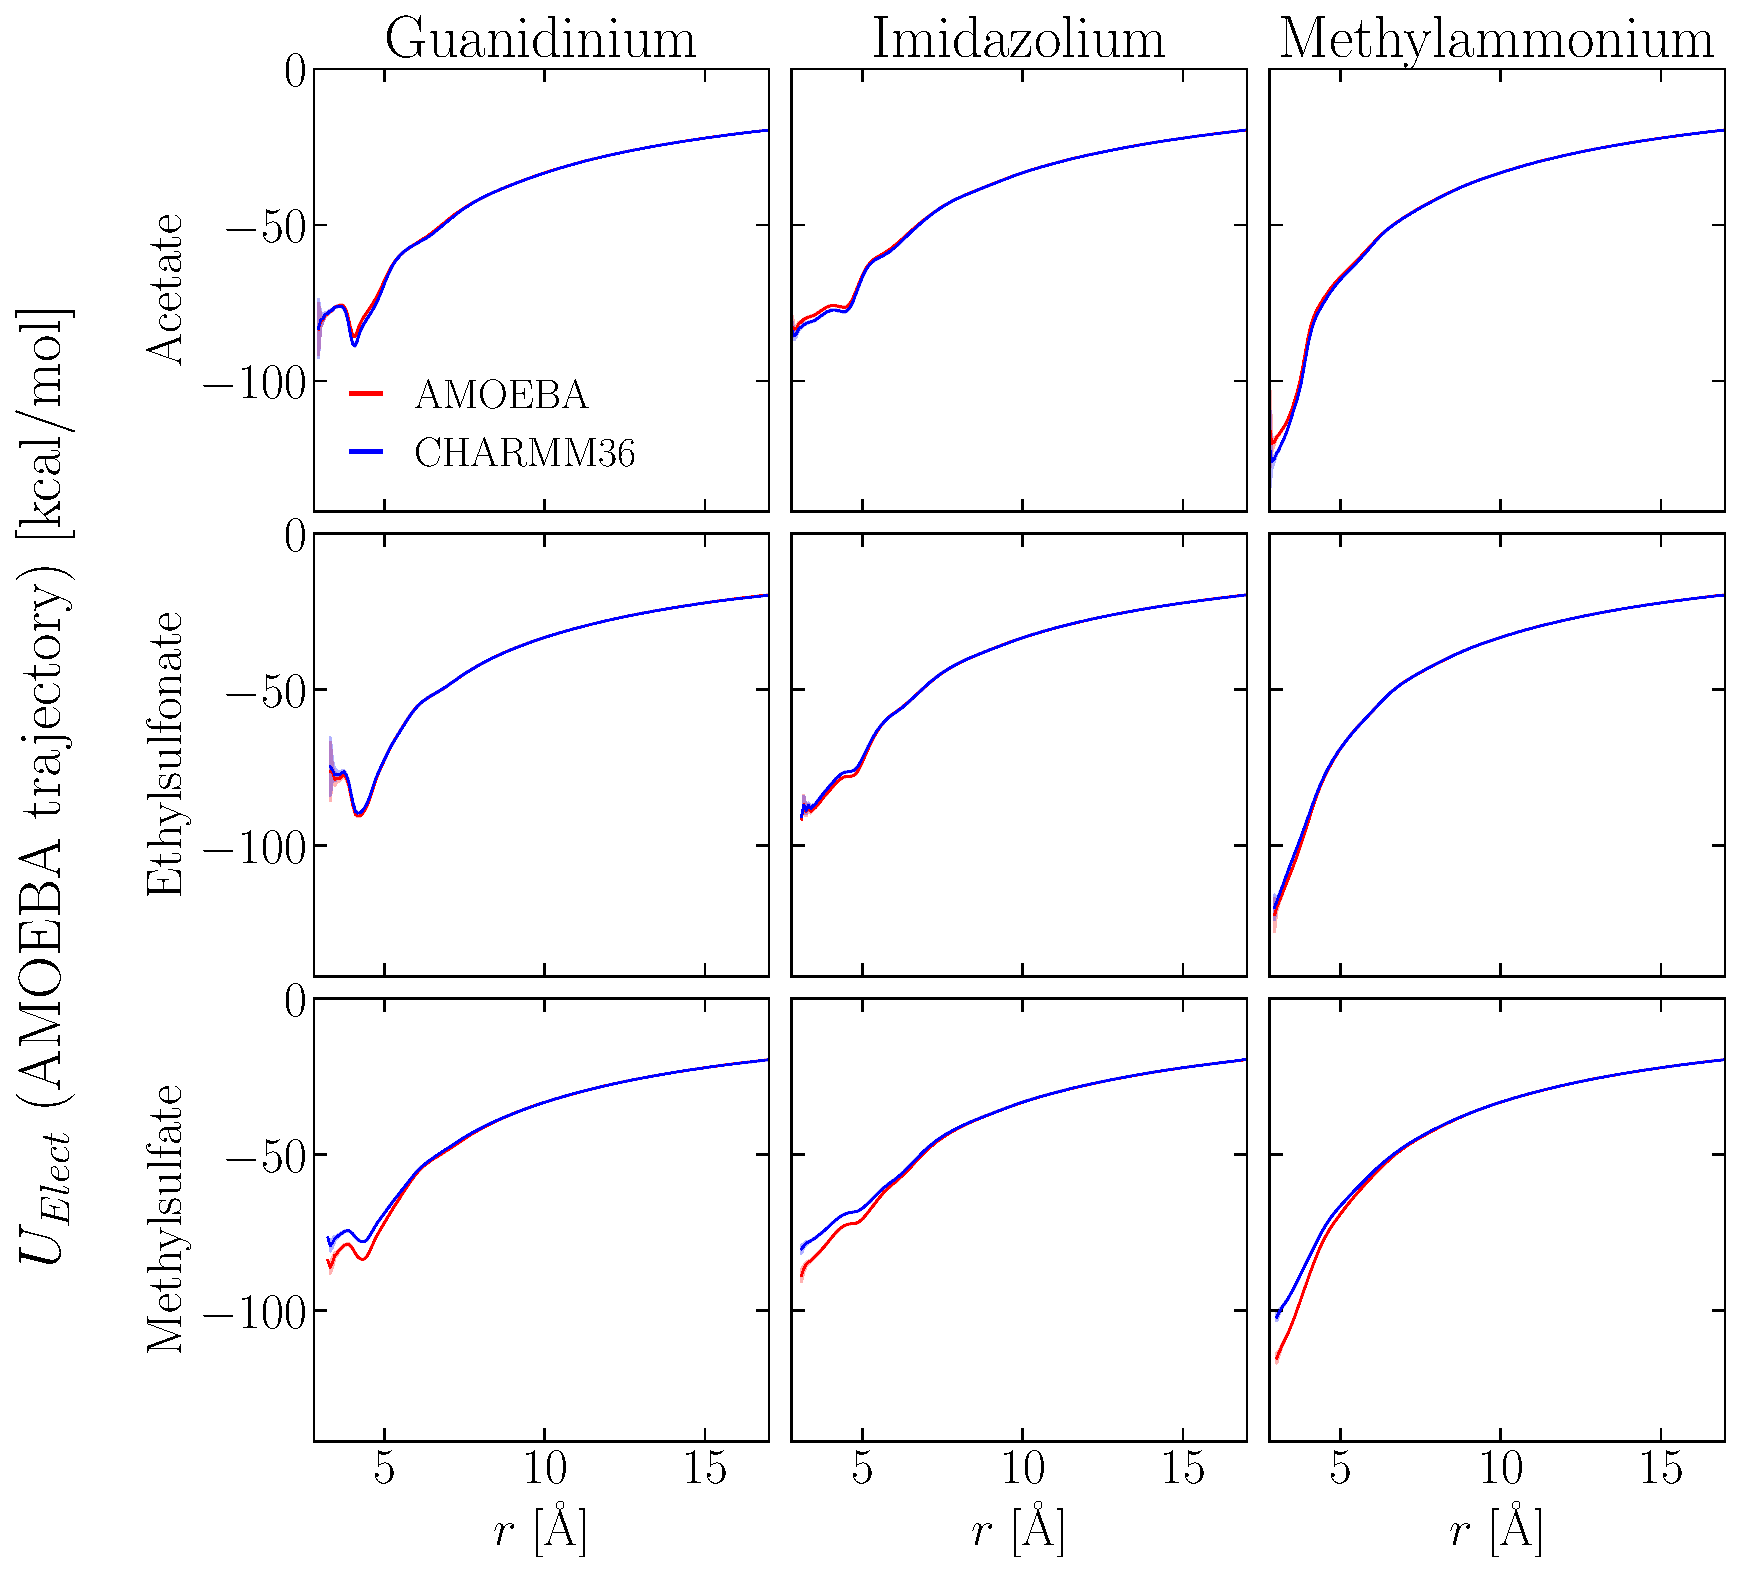
\includegraphics[width=1\columnwidth]{images/cross_ff_analysis_elect_traj_generated_by_amoeba.pdf}
        \caption{Permanent electrostatic contributions ($U_{Elect}$) to the \emph{in vacuo} interaction energy between anion-cation pairs in configurations from the AMOEBA simulation trajectory when retrospectively analyzed using the AMOEBA and CHARMM36 force fields. Shaded regions represent $2\times$ the standard error of the mean.}
        \label{fig:cross_ff_elect}
    \end{center}
    \end{figure}

    \begin{figure}[H]
    \begin{center}
        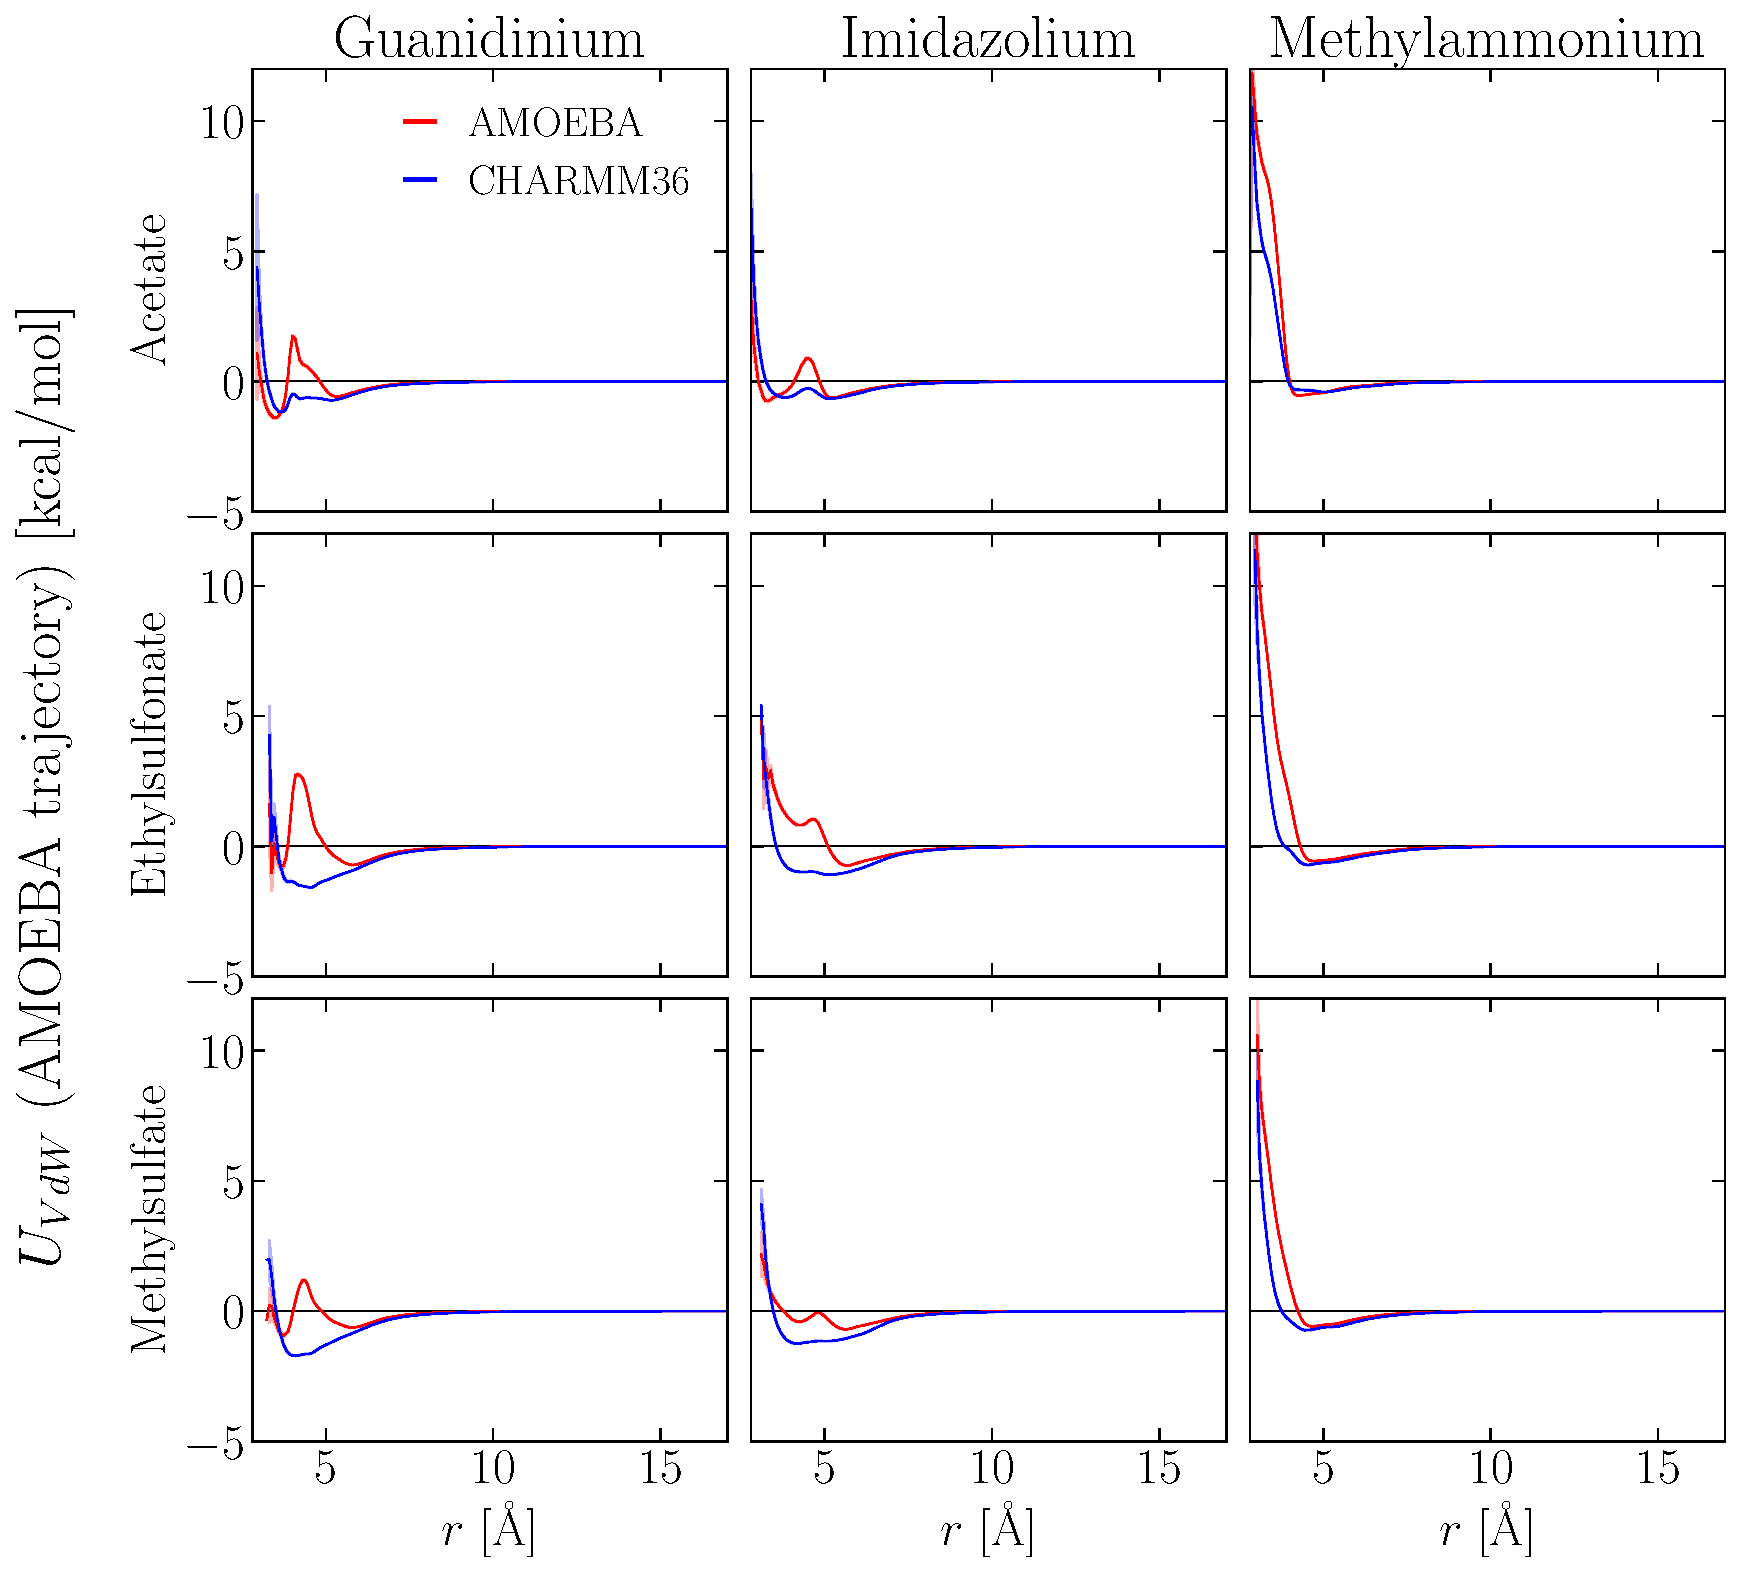
\includegraphics[width=1\columnwidth]{images/cross_ff_analysis_vdw_traj_generated_by_amoeba.pdf}
        \caption{Van der Waals contributions ($U_{VdW}$) to the \emph{in vacuo} interaction energy between anion-cation pairs in configurations from the AMOEBA simulation trajectory when retrospectively analyzed using the AMOEBA and CHARMM36 force fields. Shaded regions represent $2\times$ the standard error of the mean.}
        \label{fig:cross_ff_vdw}
    \end{center}
    \end{figure}

    \begin{figure}[H]
    \begin{center}
        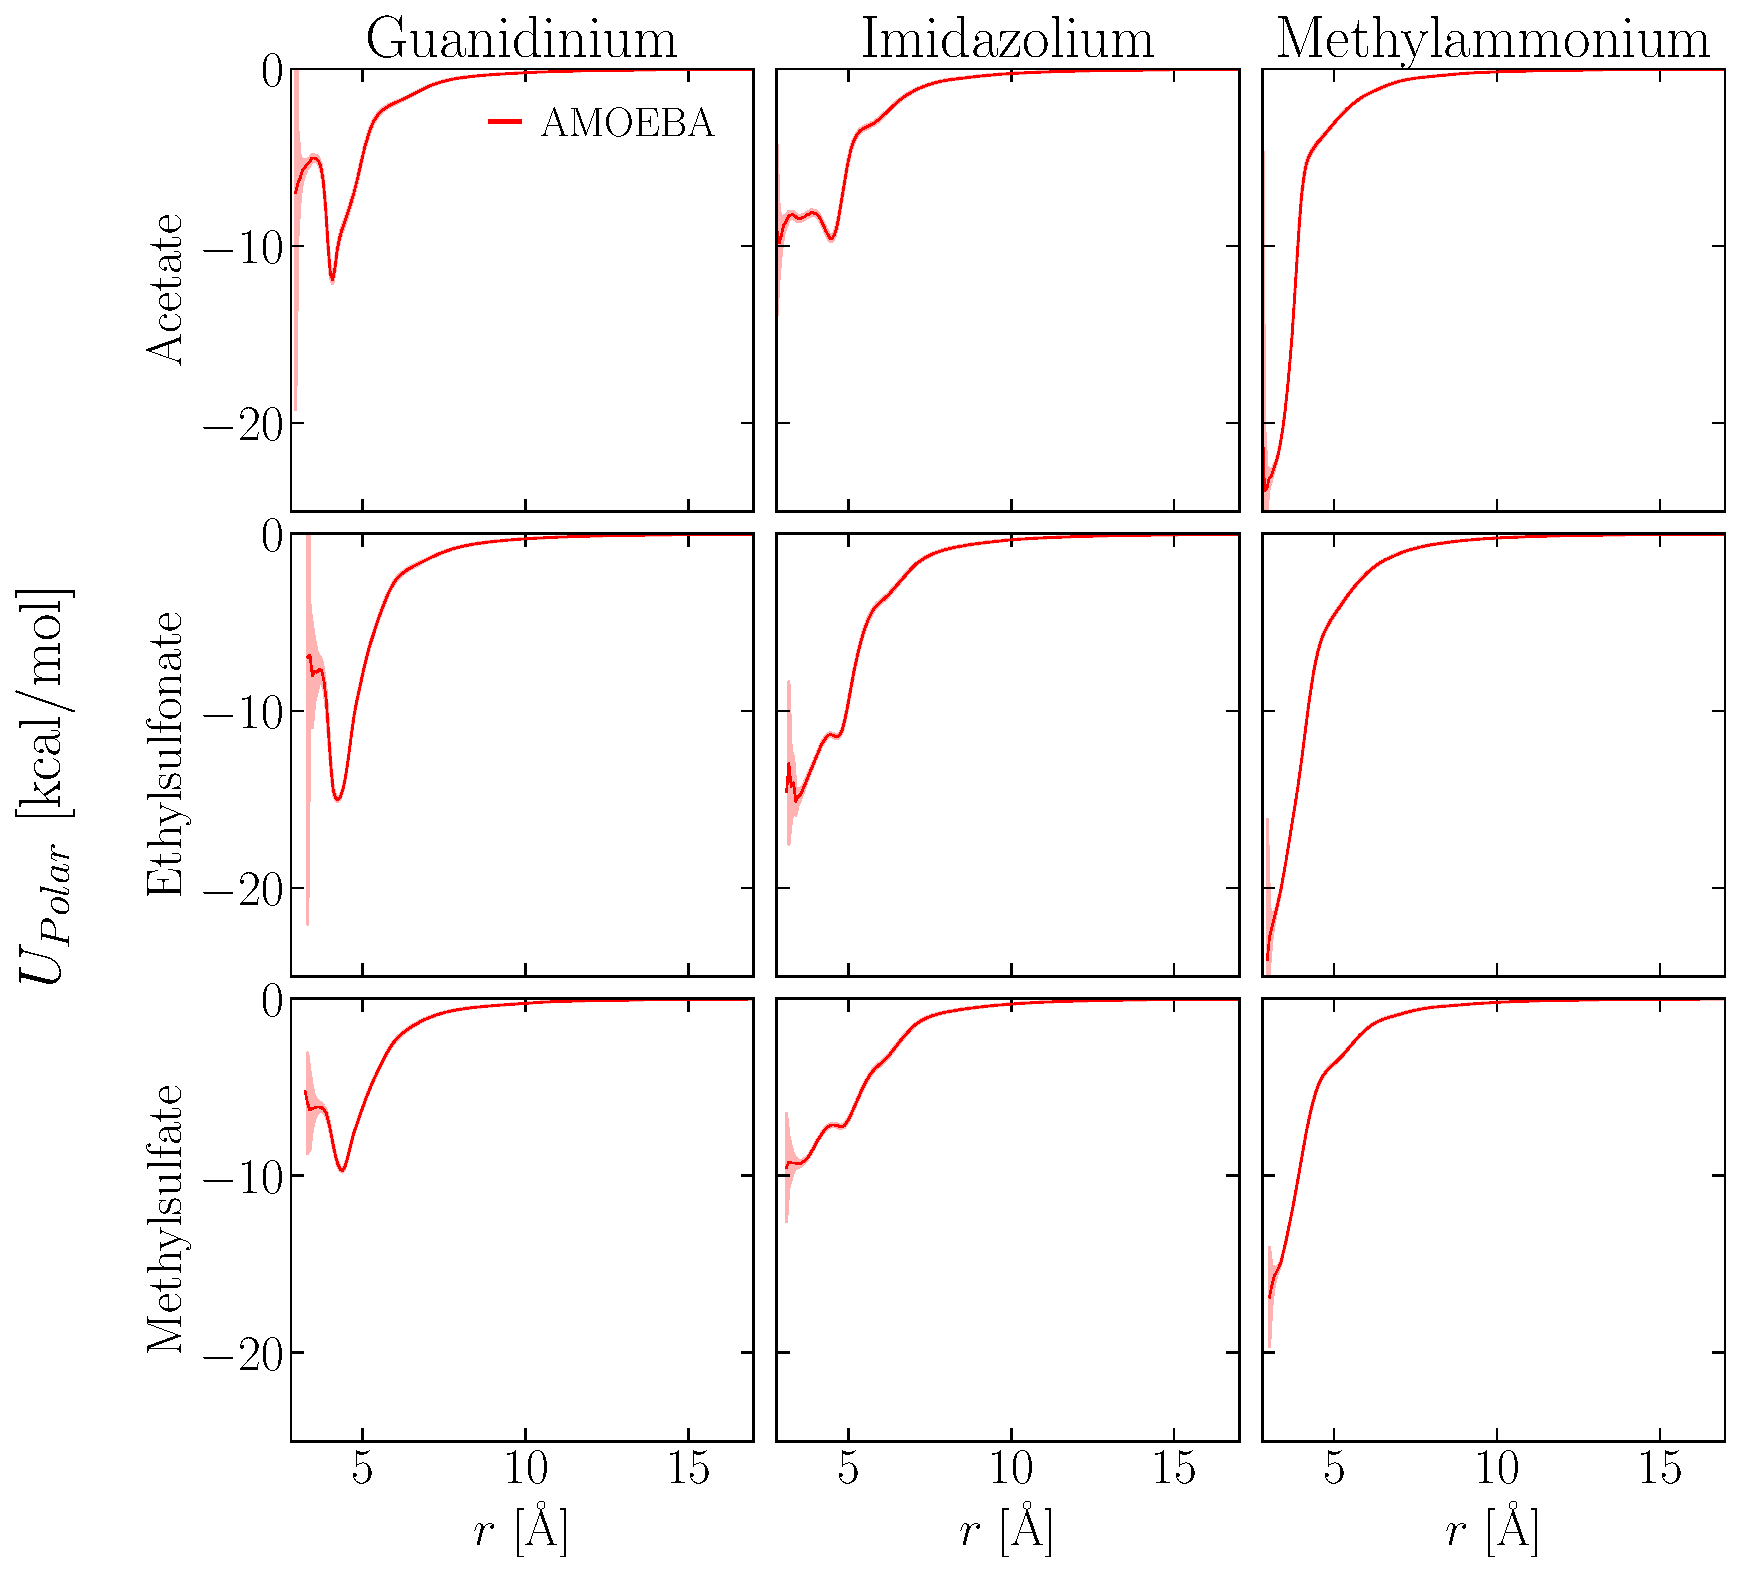
\includegraphics[width=1\columnwidth]{images/energy_conts_polar.pdf}
        \caption{Estimated contribution of polarization ($U_{Polar}$) to the \emph{in vacuo} interaction energy between anion-cation pairs in configurations from the AMOEBA simulation trajectory when retrospectively analyzed using the AMOEBA force field. Shaded regions represent $2\times$ the standard error of the mean. (There are no polarization contributions in CHARMM36, so $U_{Polar}$ is trivially zero for that force field.)}
        \label{fig:energy_conts_polar}
    \end{center}
    \end{figure}

    \begin{figure}[H]
    \begin{center}
        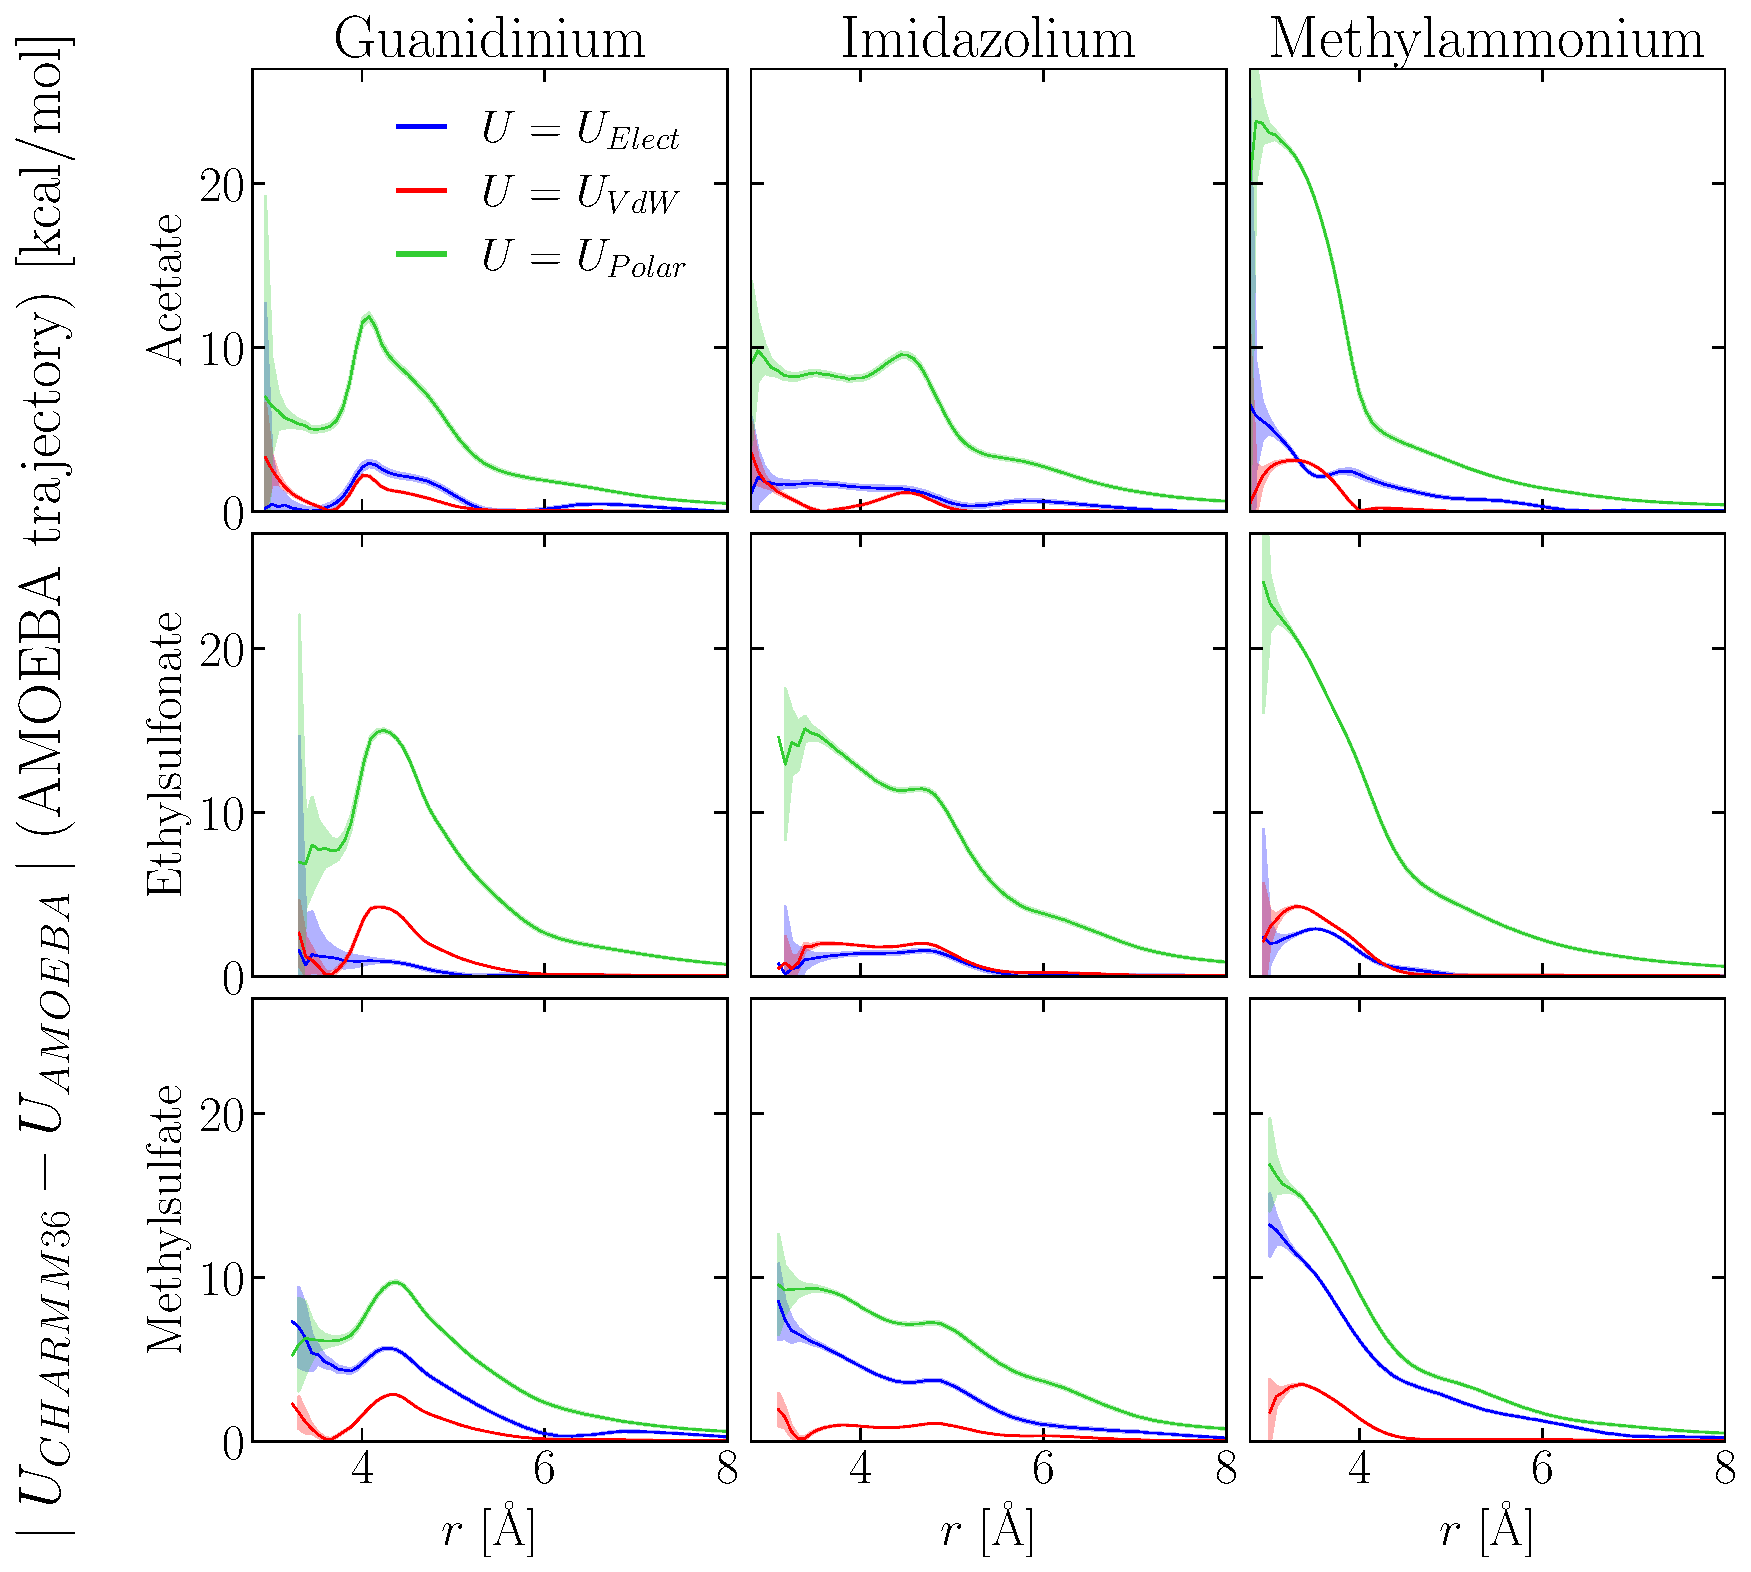
\includegraphics[width=1\columnwidth]{images/cross_ff_analysis_energy_cont_diff.pdf}
        \caption{Magnitude of the differences between \emph{in vacuo} interaction energy contributions for anion-cation pairs in configurations from the AMOEBA simulation trajectory when retrospectively analyzed using the AMOEBA and CHARMM36 force fields. Notice that polarization stabilizes ion-pairing interactions \emph{in vacuo}. Shaded regions represent $2\times$ the standard error of the mean. (In the computation of differences in $U_{Polar}$, $U_{CHARMM36}$ is trivially zero.) }
        \label{fig:cross_ff_diff}
    \end{center}
    \end{figure}




    \subsection{Generating-FF analysis results}

    \begin{figure}[H]
    \begin{center}
        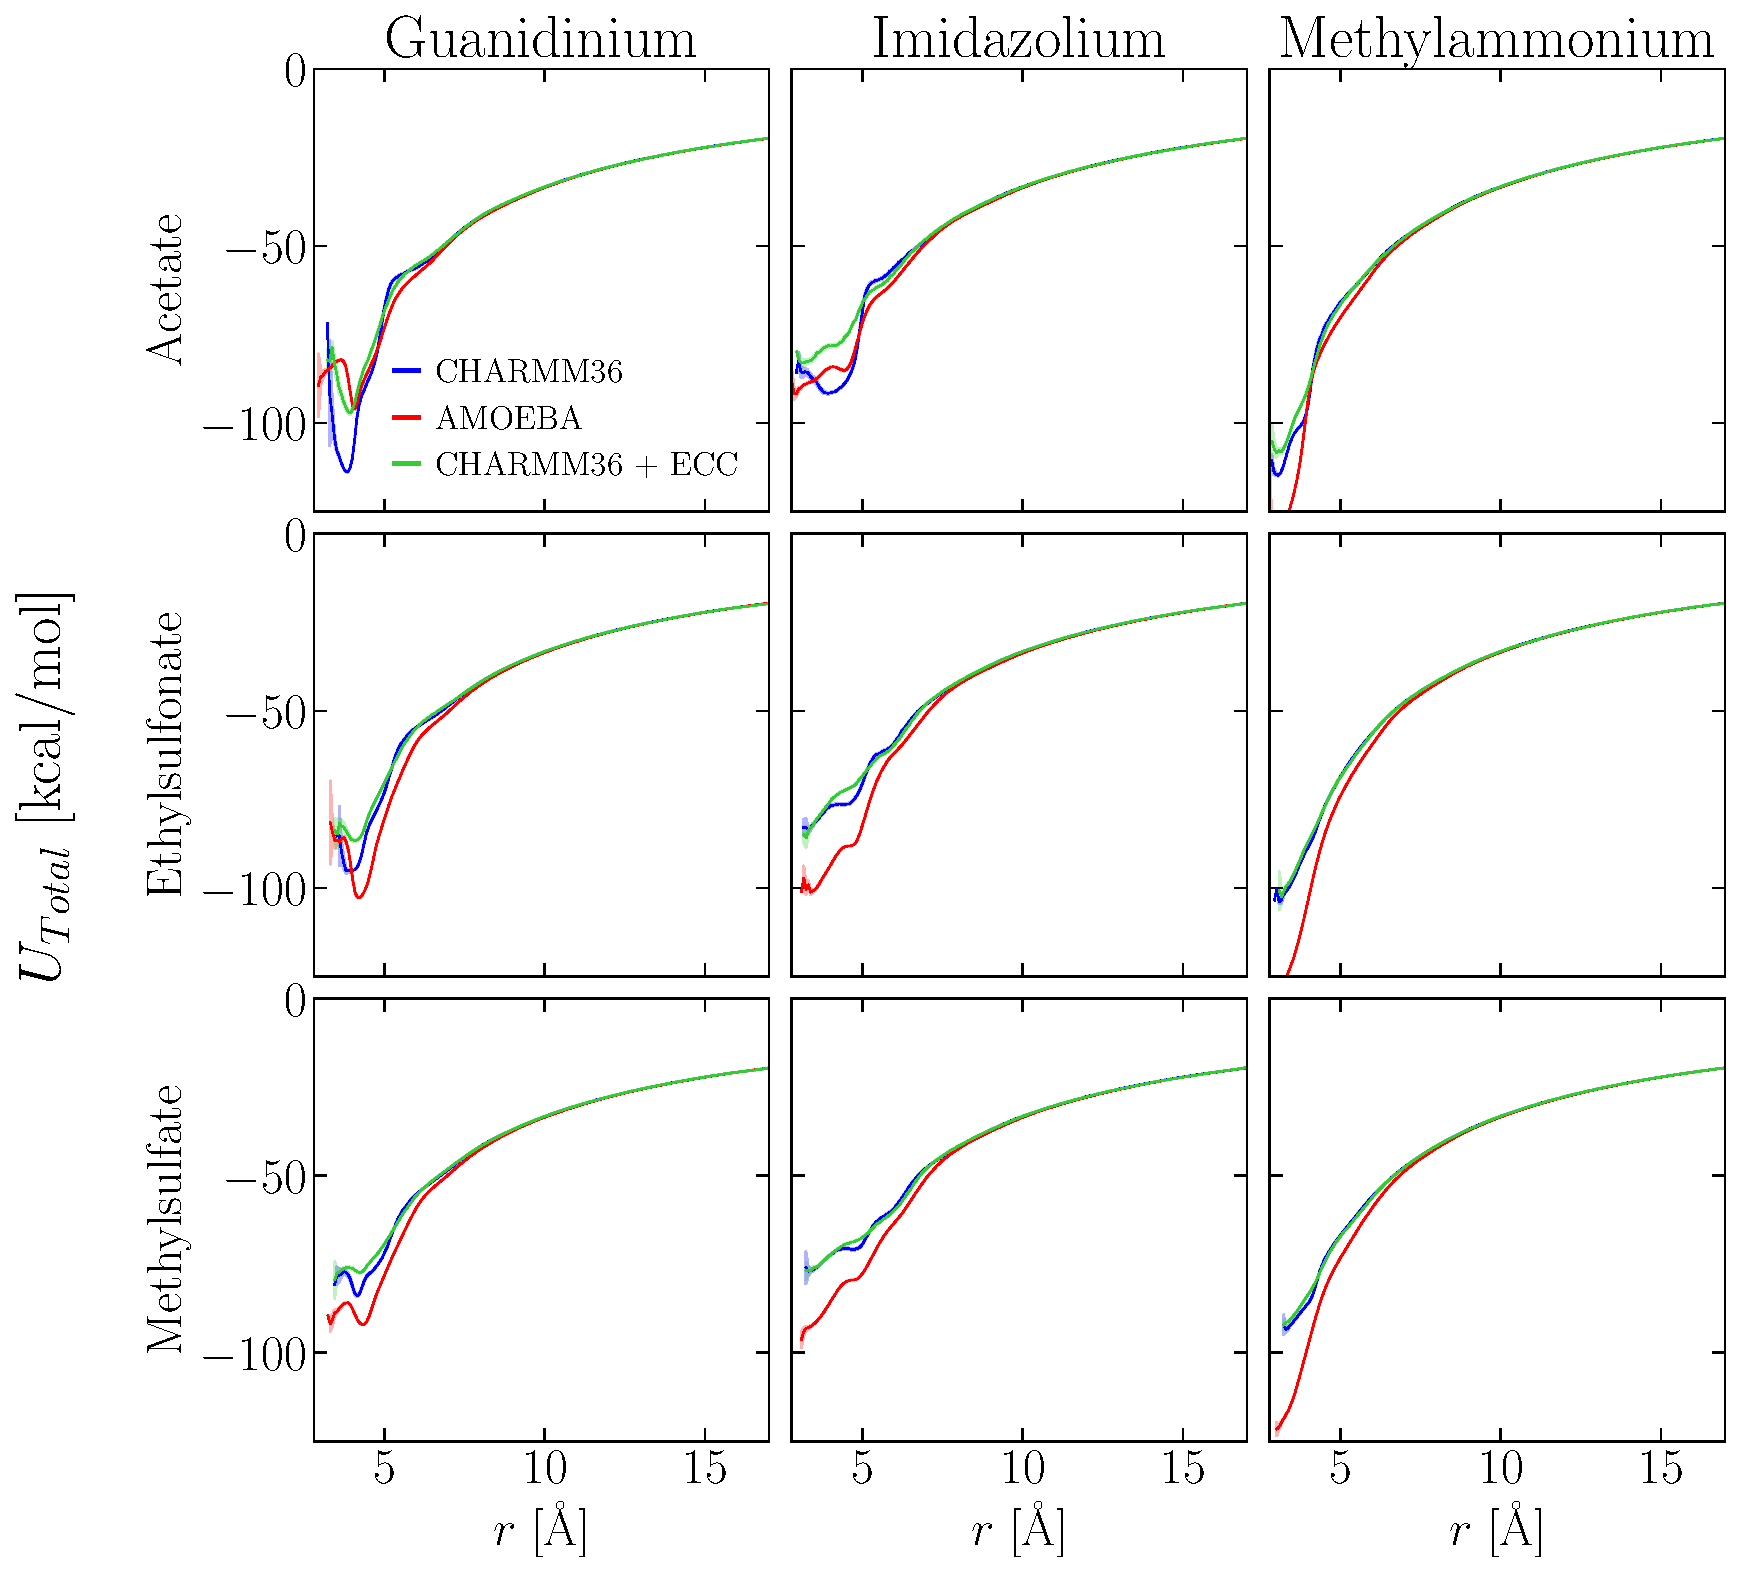
\includegraphics[width=1\columnwidth]{images/energy_conts_direct.pdf}
        \caption{Total \emph{in vacuo} interaction energy between anion-cation pairs, computed as $U_{Total} = U_{Elect} + U_{VdW} + U_{Polar}$ in the separate simulation trajectories using the trajectory-generating force field, where $U_{Elect}$ has been scaled up by $1/0.75^2$ for the CHARMM36~+~ECC results. Shaded regions represent $2\times$ the standard error of the mean.}
        \label{fig:energy_conts_direct}
    \end{center}
    \end{figure}

    \begin{figure}[H]
    \begin{center}
        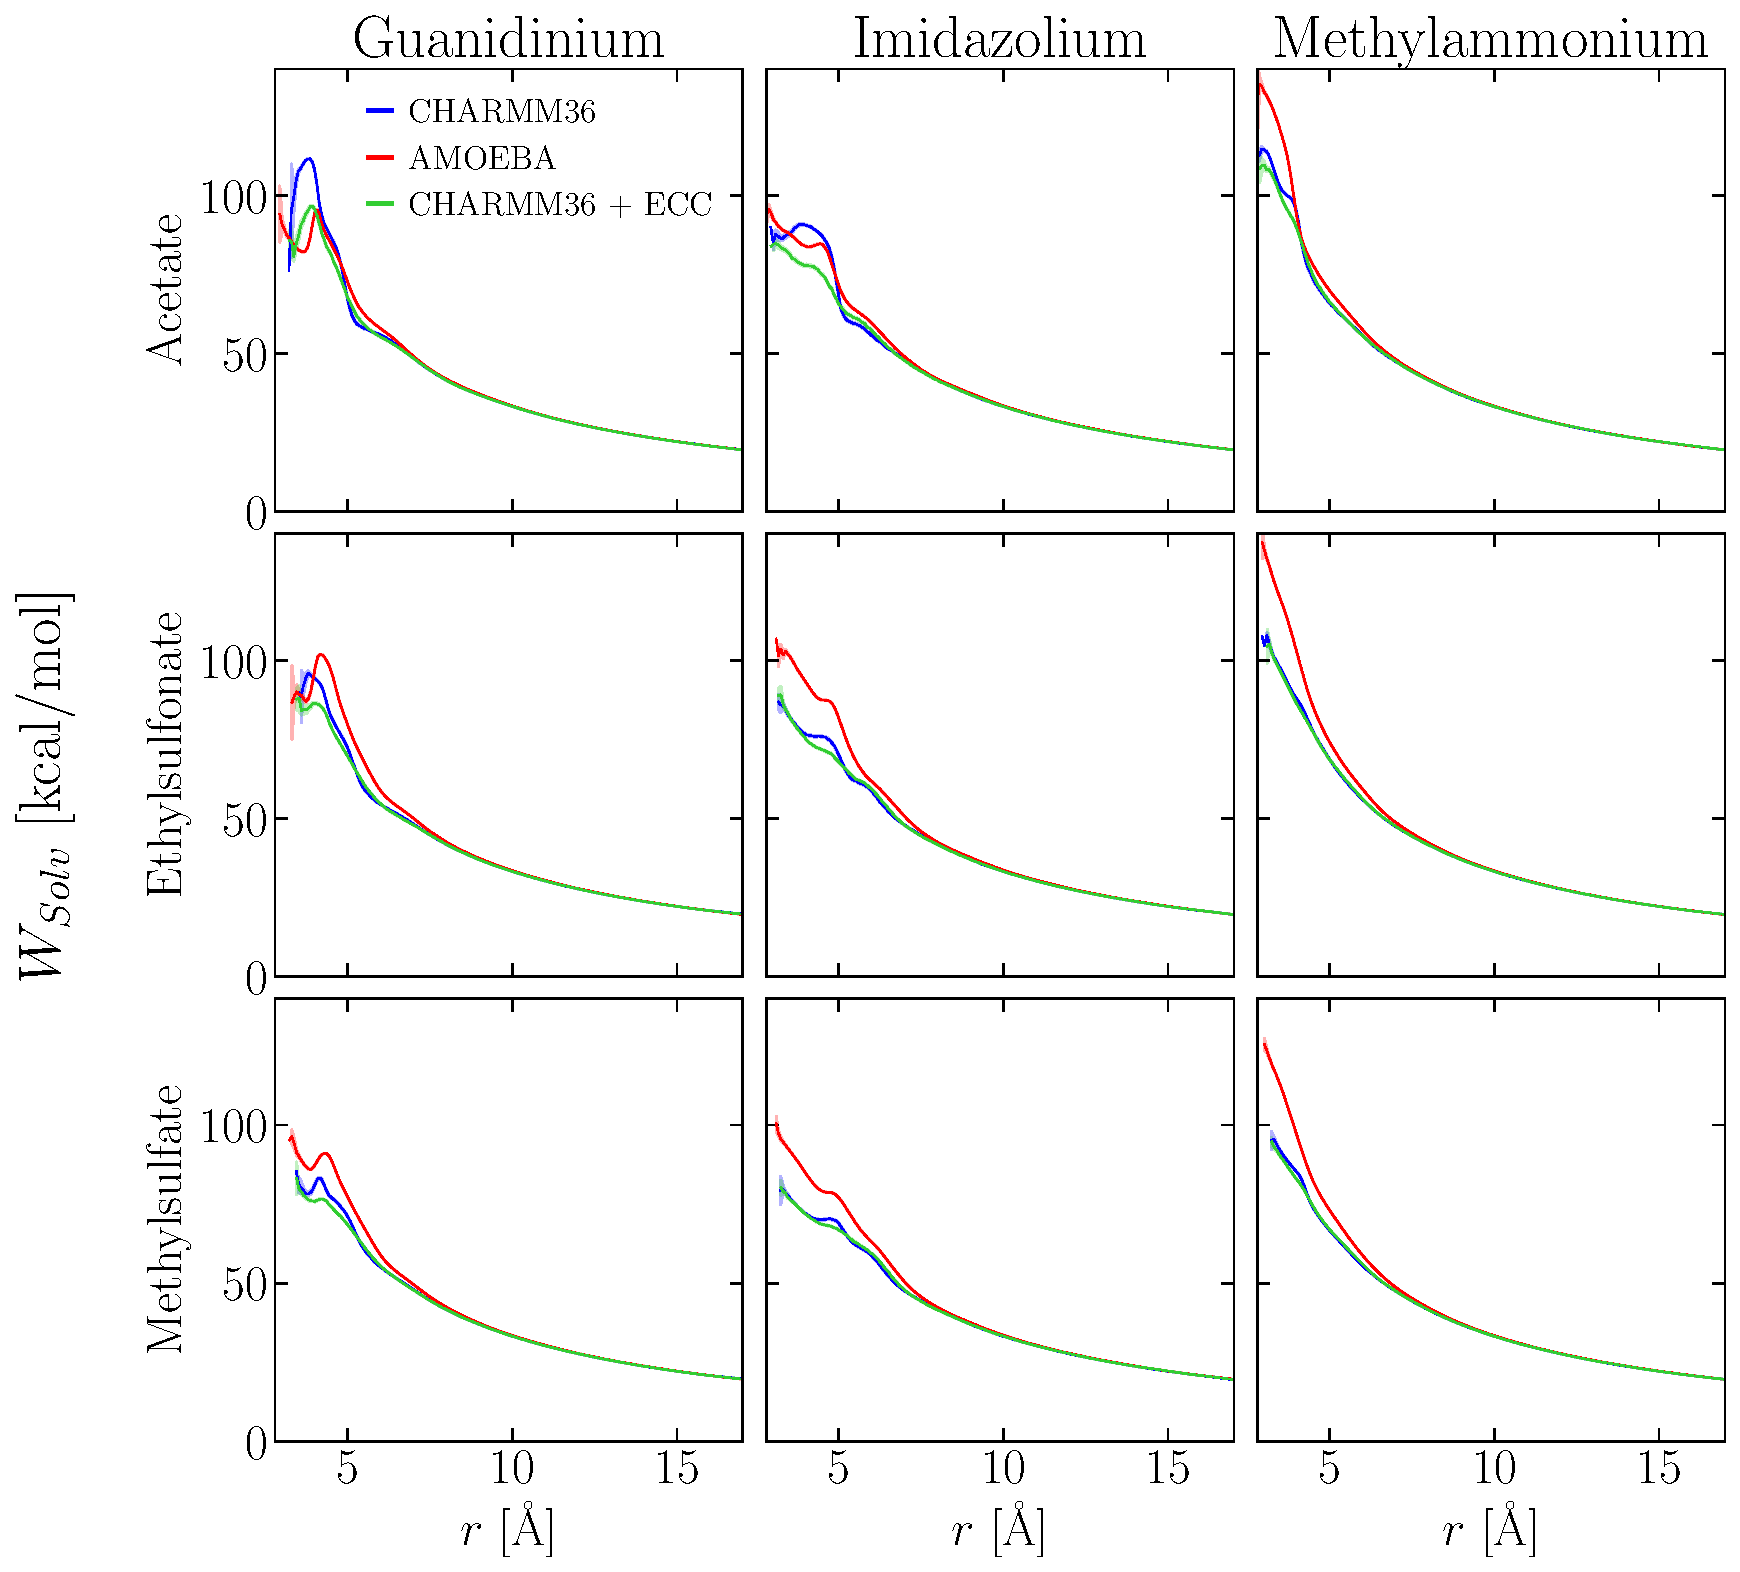
\includegraphics[width=1\columnwidth]{images/energy_conts_w_solv.pdf}
        \caption{Estimated solvent opposition to ion-pair association, inferred as $W_{Solv}~=~\text{PMF}~-~U_{Total}$ in the separate simulation trajectories using the trajectory-generating force field. $U_{Elect}$ was scaled up by $1/0.75^2$ in the computation of $U_{Total}$ for the CHARMM36 + ECC results. Shaded regions represent $2\times$ the standard error of the mean.}
        \label{fig:energy_conts_w_solv}
    \end{center}
    \end{figure}
    

    \begin{figure}[H]
    \begin{center}
        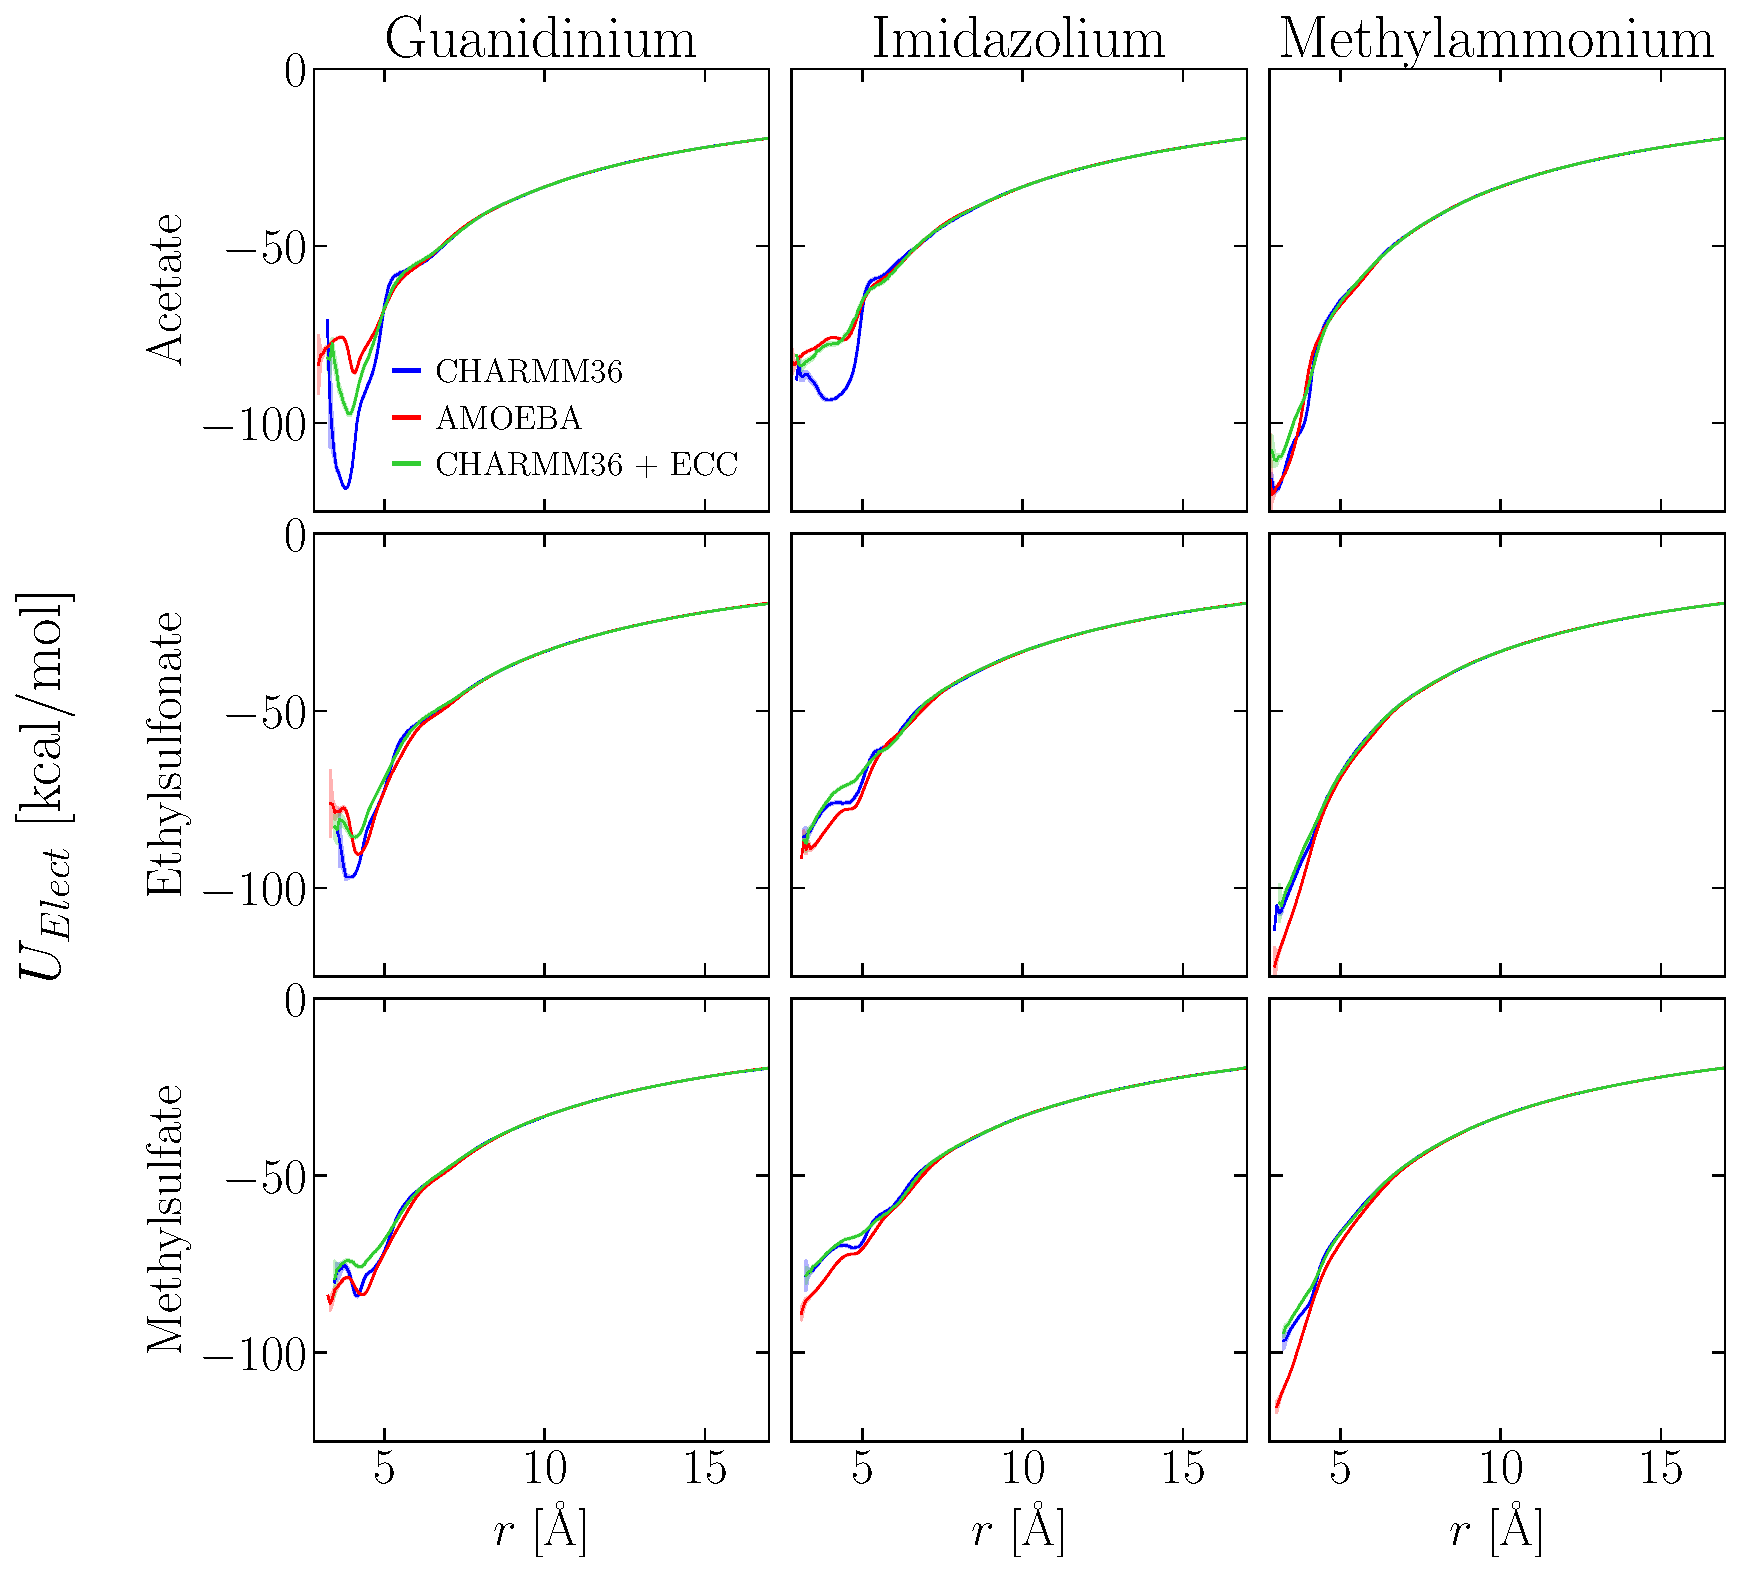
\includegraphics[width=1\columnwidth]{images/energy_conts_elect.pdf}
        \caption{Permanent electrostatic contributions ($U_{Elect}$) to the \emph{in vacuo} interaction energy between anion-cation pairs in configurations from the different simulation trajectories when analyzed using the trajectory-generating force field. The CHARMM36 + ECC results have been scaled by a factor of $1/0.75^2$ to facilitate comparison. Shaded regions represent $2\times$ the standard error of the mean.}
        \label{fig:energy_conts_elect}
    \end{center}
    \end{figure}

    \begin{figure}[H]
    \begin{center}
        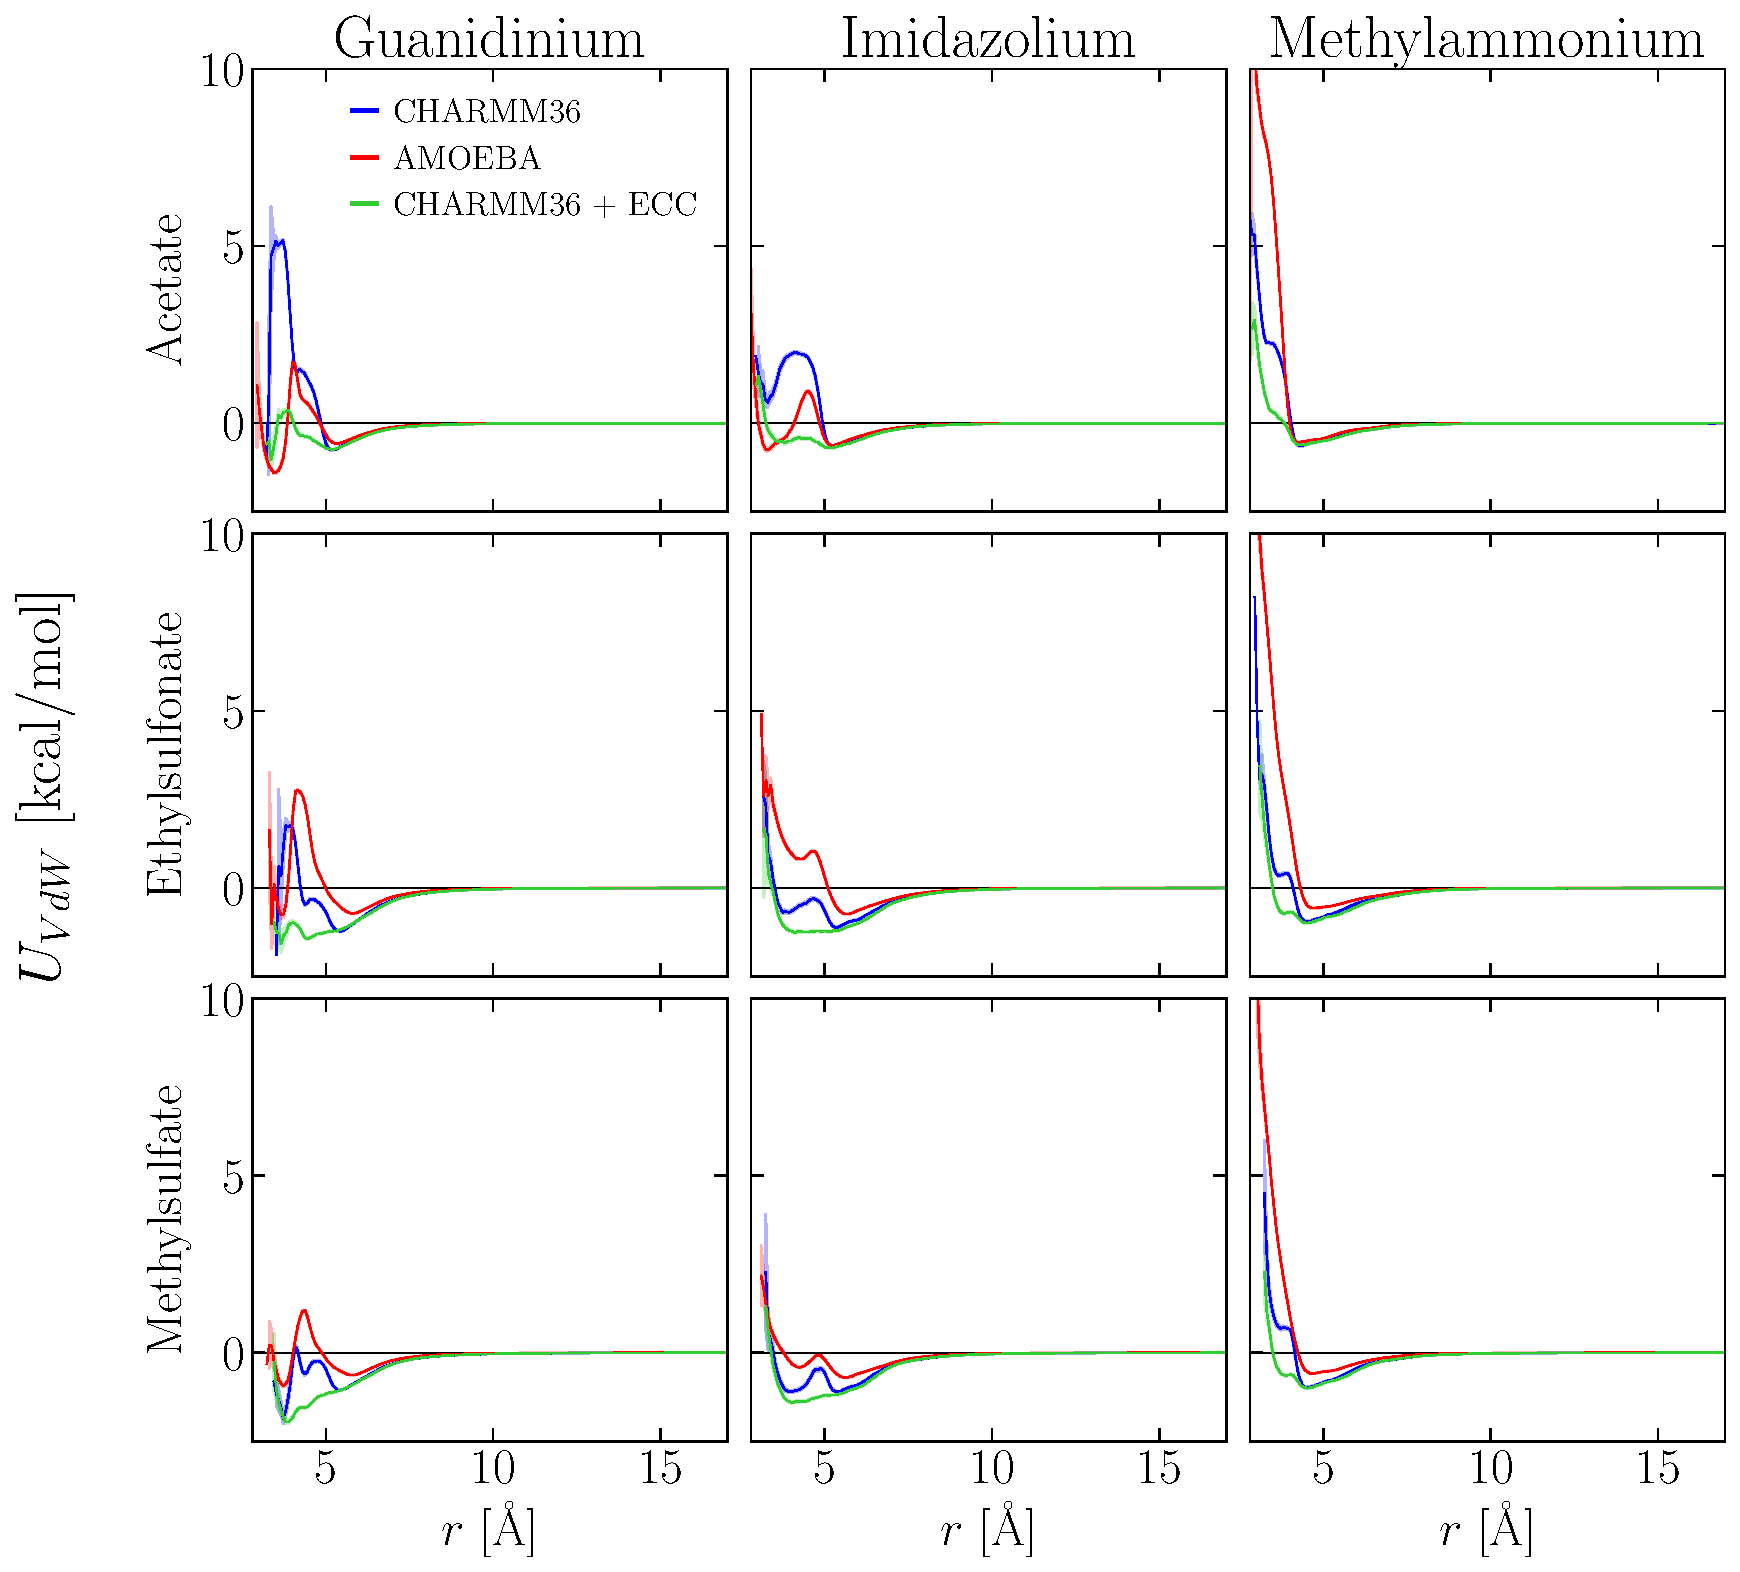
\includegraphics[width=1\columnwidth]{images/energy_conts_vdw.pdf}
        \caption{Van der Waals contributions ($U_{VdW}$) to the \emph{in vacuo} interaction energy between anion-cation pairs in configurations from the different simulation trajectories when analyzed using the trajectory-generating force field. Shaded regions represent $2\times$ the standard error of the mean.}
        \label{fig:energy_conts_vdw}
    \end{center}
    \end{figure}

    \begin{figure}[H]
    \begin{center}
        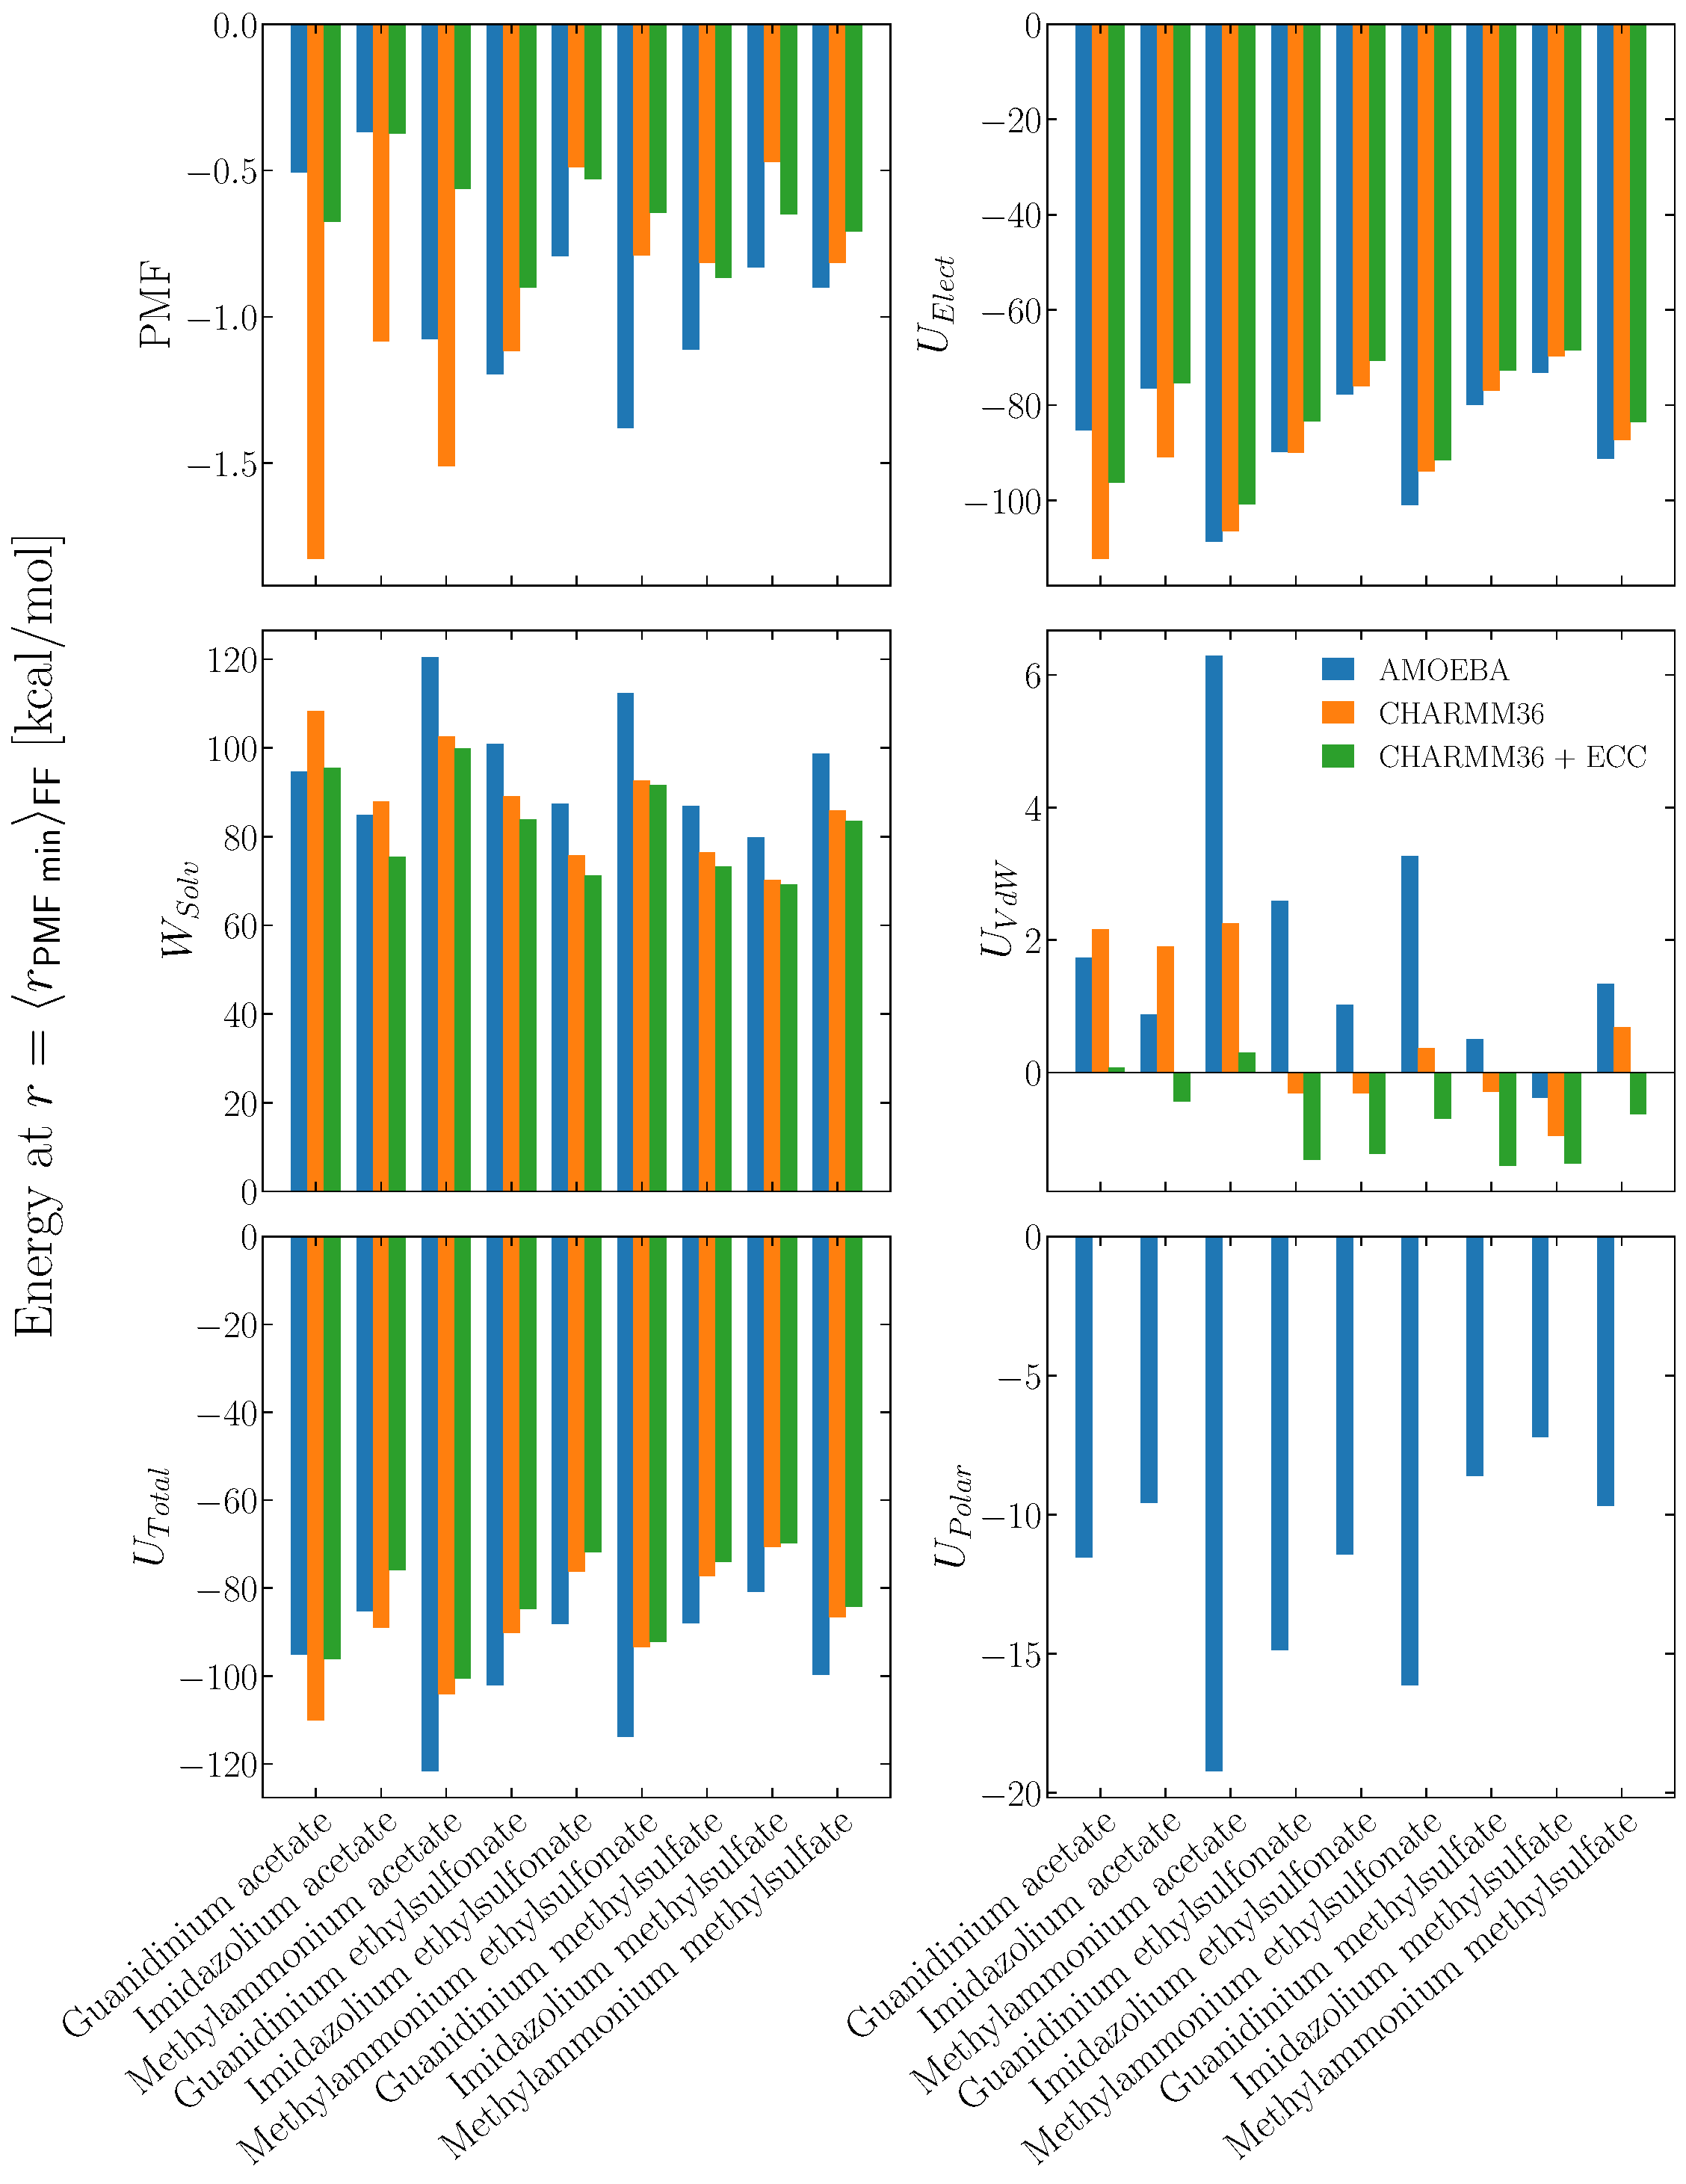
\includegraphics[width=0.9\columnwidth]{images/energy_cont_bar_plots.pdf}
        \caption{Interaction energy contributions near the PMF minimum (i.e., at the average $r_{PMF \; min}$ of the three force fields), computed from the separate simulation trajectories using the trajectory-generating force field. $U_{Elect}$ has been scaled up by $1/0.75^2$ for the CHARMM36~+~ECC results in the presentation of $U_{Elect}$, $U_{Total}$ and $W_{Solv}$.}
        \label{fig:energy_cont_bar_plots}
    \end{center}
    \end{figure}





    
    \begin{landscape}
    \section{Maps of configurational sampling}
    \subsection{3D plots}
    
    \begin{figure}[H]
    \begin{center}
        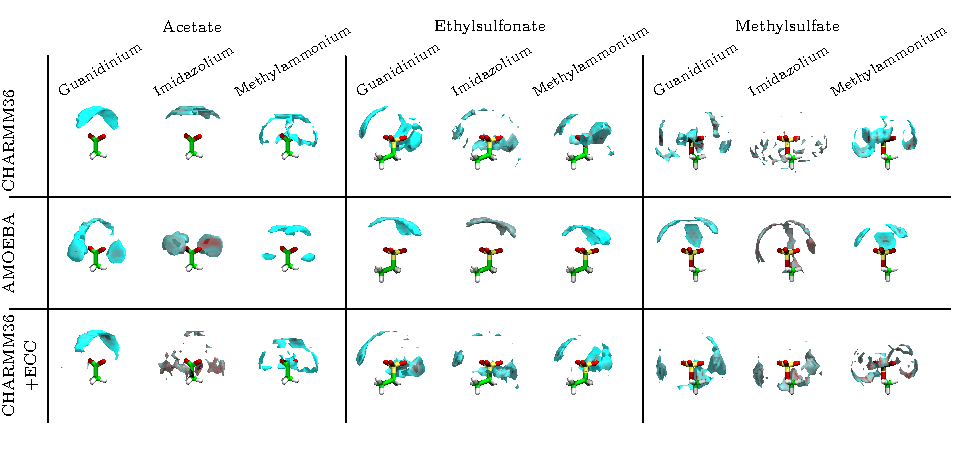
\includegraphics[width=1.48\textwidth]{images/fig_heatmaps_anions.pdf}
        \caption{Spaces of most frequent cation sampling around anions. The shaded regions represent the top 1000 voxels in a cubic mesh (defined relative to the anion with a grid spacing of 0.5~\AA) where the sampling frequency was greatest for the ``central" cation atoms that are distinguished by blue circles in Figure~1. (Images were created using VMD.\cite{Humphrey1996})}
        \label{fig:3D_anions}
    \end{center}
    \end{figure}
    
    \begin{figure}[H]
    \begin{center}
        \includegraphics[width=1.48\textwidth]{images/fig_heatmaps_cations.pdf}
        \caption{Spaces of most frequent anion sampling around cations. The shaded regions represent the top 1000 voxels in a cubic mesh (defined relative to the cation with a grid spacing of 0.5~\AA) where the sampling frequency was greatest for the ``central" anion atoms that are distinguished by grey circles in Figure~1. (Images were created using VMD.\cite{Humphrey1996})}
        \label{fig:3D_cations}
    \end{center}
    \end{figure}
    
    \end{landscape}




    
    \subsection{Coordinate definitions for heat maps}

    The separation distance $r = | \vec{r_1} |$ between a given anion-cation pair was defined using the central atoms that are distinguished in Figure 1, where grey and blue circles are used to distinguish the central atoms in anions and cations, respectively.
    % HARD CODED
    For clarity these atoms are also listed in Table~\ref{tab:coordinates} using the CHARMM36 atom names that are shown in Figure~\ref{fig:charmm_atom_names}. Angular coordinates $\theta$ and $\alpha$ were also defined to provide measures of the anion orientation relative to the cation and of the cation orientation relative to the anion, respectively. The definition of these coordinates depends on the ion pair and is explained in Table~\ref{tab:coordinates}.
    
    \begin{figure}[H]
    \begin{center}
        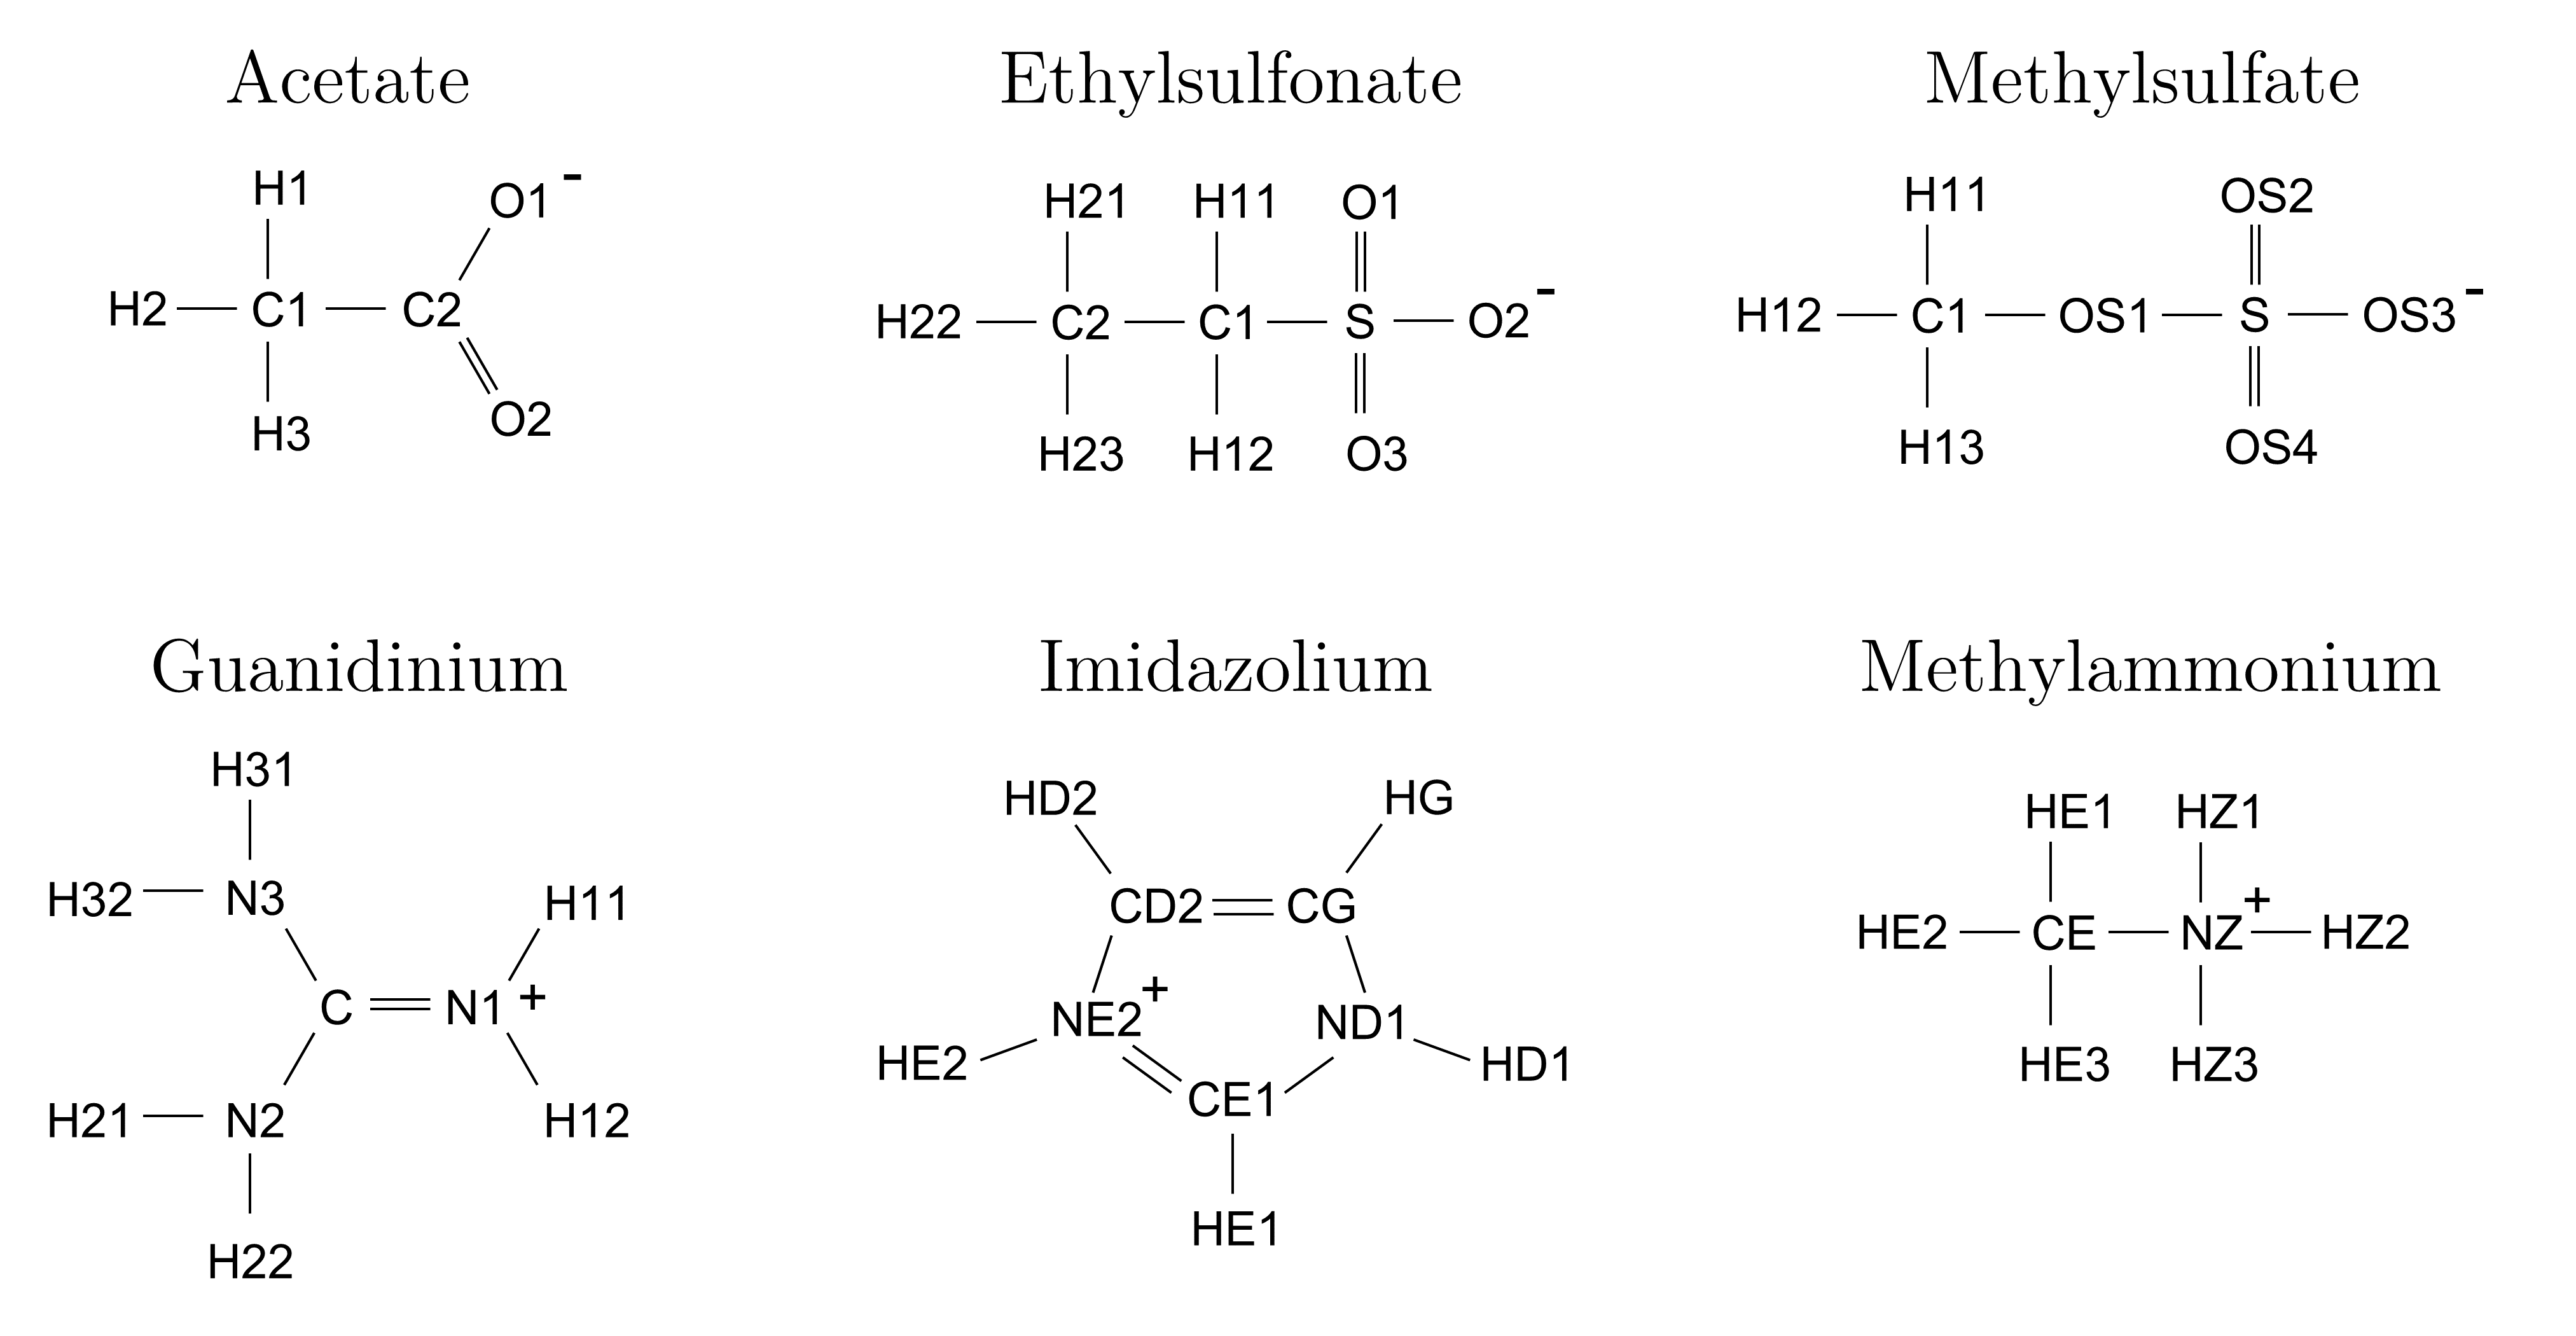
\includegraphics[width=\columnwidth]{images/charmm_atom_names_2.png}
        \caption{Ion structures with atom names from the CHARMM36 convention,\cite{Huang2013} where the first letter represents the element.}
        \label{fig:charmm_atom_names}
    \end{center}
    \end{figure}

    \begin{table}[H]
    \caption{Coordinate definitions for each anion-cation pair, where $A_{X}^{-}C_{Y}^{+}$ for example refers to the vector pointing from atom $X$ in the anion to atom $Y$ in the cation (cf. Figure~\ref{fig:charmm_atom_names} for atom names). The coordinate $r = | \vec{r_1} |$ represents the separation distance between the respective central atoms of the anion and the cation. The coordinate $\theta$ is computed as the angle between $\vec{r_1}$ and $\vec{r_2}$ and provides a measure of the anion orientation relative to the cation. The definition of $\alpha$ depends on the cation and provides a measure of the cation orientation relative to the anion.}
    \label{tab:coordinates}
    \centering
    \renewcommand{\arraystretch}{1.5}
    \begin{tabular}{>{\centering\arraybackslash}m{0.2\linewidth} | >{\centering\arraybackslash}m{0.17\linewidth} | >{\centering\arraybackslash}m{0.09\linewidth} | >{\centering\arraybackslash}m{0.09\linewidth} | >{\centering\arraybackslash}m{0.35\linewidth}}
    
    Cation         & Anion          & $\vec{r_1}$     & $\vec{r_2}$    & $\alpha$                                                                    \\ \hline
    Guanidinium    & Acetate        & $A_{C2}^{-}C_{C}^{+}$   & $A_{C2}^{-}A_{C1}^{-}$ & Angle formed by $\vec{r_1}$ and the plane defined by $C_{N1}^{+}C_{N2}^{+}C_{N3}^{+}$ \\
    Guanidinium    & Ethylsulfonate & $A_{S}^{-}C_{C}^{+}$    & $A_{S}^{-}A_{C1}^{-}$  & Angle formed by $\vec{r_1}$ and the plane defined by $C_{N1}^{+}C_{N2}^{+}C_{N3}^{+}$ \\
    Guanidinium    & Methylsulfate  & $A_{S}^{-}C_{C}^{+}$    & $A_{S}^{-}A_{OS1}^{-}$ & Angle formed by $\vec{r_1}$ and the plane defined by $C_{N1}^{+}C_{N2}^{+}C_{N3}^{+}$ \\ \hline
    Imidazolium    & Acetate        & $A_{C2}^{-}C_{CE1}^{+}$ & $A_{C2}^{-}A_{C1}^{-}$ & Angle formed by $\vec{r_1}$ and the plane defined by $C_{CG}^{+}C_{CD2}^{+}C_{CE1}^{+}$  \\
    Imidazolium    & Ethylsulfonate & $A_{S}^{-}C_{CE1}^{+}$  & $A_{S}^{-}A_{C1}^{-}$  & Angle formed by $\vec{r_1}$ and the plane defined by $C_{CG}^{+}C_{CD2}^{+}C_{CE1}^{+}$  \\
    Imidazolium    & Methylsulfate  & $A_{S}^{-}C_{CE1}^{+}$  & $A_{S}^{-}A_{OS1}^{-}$ & Angle formed by $\vec{r_1}$ and the plane defined by $C_{CG}^{+}C_{CD2}^{+}C_{CE1}^{+}$  \\ \hline
    Methylammonium & Acetate        & $A_{C2}^{-}C_{NZ}^{+}$  & $A_{C2}^{-}A_{C1}^{-}$ & Torsion angle formed by $C_{CE}^{+}C_{NZ}^{+}A_{C2}^{-}A_{C1}^{-}$ \\
    Methylammonium & Ethylsulfonate & $A_{S}^{-}C_{NZ}^{+}$   & $A_{S}^{-}A_{C1}^{-}$  & Torsion angle formed by $C_{CE}^{+}C_{NZ}^{+}A_{S}^{-}A_{C1}^{-}$ \\
    Methylammonium & Methylsulfate  & $A_{S}^{-}C_{NZ}^{+}$   & $A_{S}^{-}A_{OS1}^{-}$ & Torsion angle formed by $C_{CE}^{+}C_{NZ}^{+}A_{S}^{-}A_{OS1}^{-}$ 
    \end{tabular}
    \end{table}






    \newpage
    \subsection{Heat maps in the ($\theta$, $\alpha$) space for $r < R_{Shell}$}

     The angular coordinate $\alpha$ was defined to quantify the orientation of cations relative to anions. For the planar guanidinium and imidazolium molecules, values that are closer to 0\textdegree \ indicate anion interactions within the cation plane, whereas values closer to 90\textdegree \ indicate anion interactions orthogonal to the cation plane. For methylammonium, $\alpha$ represents a torsion angle, where values that are closer to 0\textdegree \ indicate the methylammonium $\ce{CH_3}$ group is spatially inline with the anion ``tail" atom that is highlighted in green in Figure~1, whereas values closer to 180\textdegree \ indicate the methylammonium $\ce{CH_3}$ is oriented away from the anion. Figures~\ref{fig:heatmap_guan}-\ref{fig:heatmap_mamm} show heat maps in the ($\theta$, $\alpha$) space for associated ion pairs ($r < R_{Shell}$). Figure~\ref{fig:heatmap_guan} shows that, as was observed from Figure~\ref{fig:3D_cations}, anion interactions within the guanidinium plane are generally preferred and this corresponds to the configurational space that in principle should be most accessible during the adsorption of a full protein onto a CEX surface. However for acetate, AMOEBA also has out-of-guanidinium-plane sampling at $\theta \sim 90$\textdegree, which is mimicked imperfectly by the ECC and seems consistent with the findings in Mason et al.\cite{Mason2019a} For imidazolium, in-plane interactions are also preferred but are less distinct (Figure~\ref{fig:heatmap_imim}). For the methylammonium systems there is generally no torsional preference in the CHARMM36 or ECC data, but there are distinct preferences in AMOEBA (Figure~\ref{fig:heatmap_mamm}). For instance the association of acetate with methylammonium favors $\alpha < 90$\textdegree \ such that the $\ce{CH_3}$ groups of both methylammonium and acetate may interact. Conversely there is a slight preference for the methylammonium $\ce{CH_3}$ group to be oriented away from the the sulfur-containing ligands, which represents the configurational space that in principle should be most accessible during protein interactions.
     
    \begin{figure}[H]
    \begin{center}
        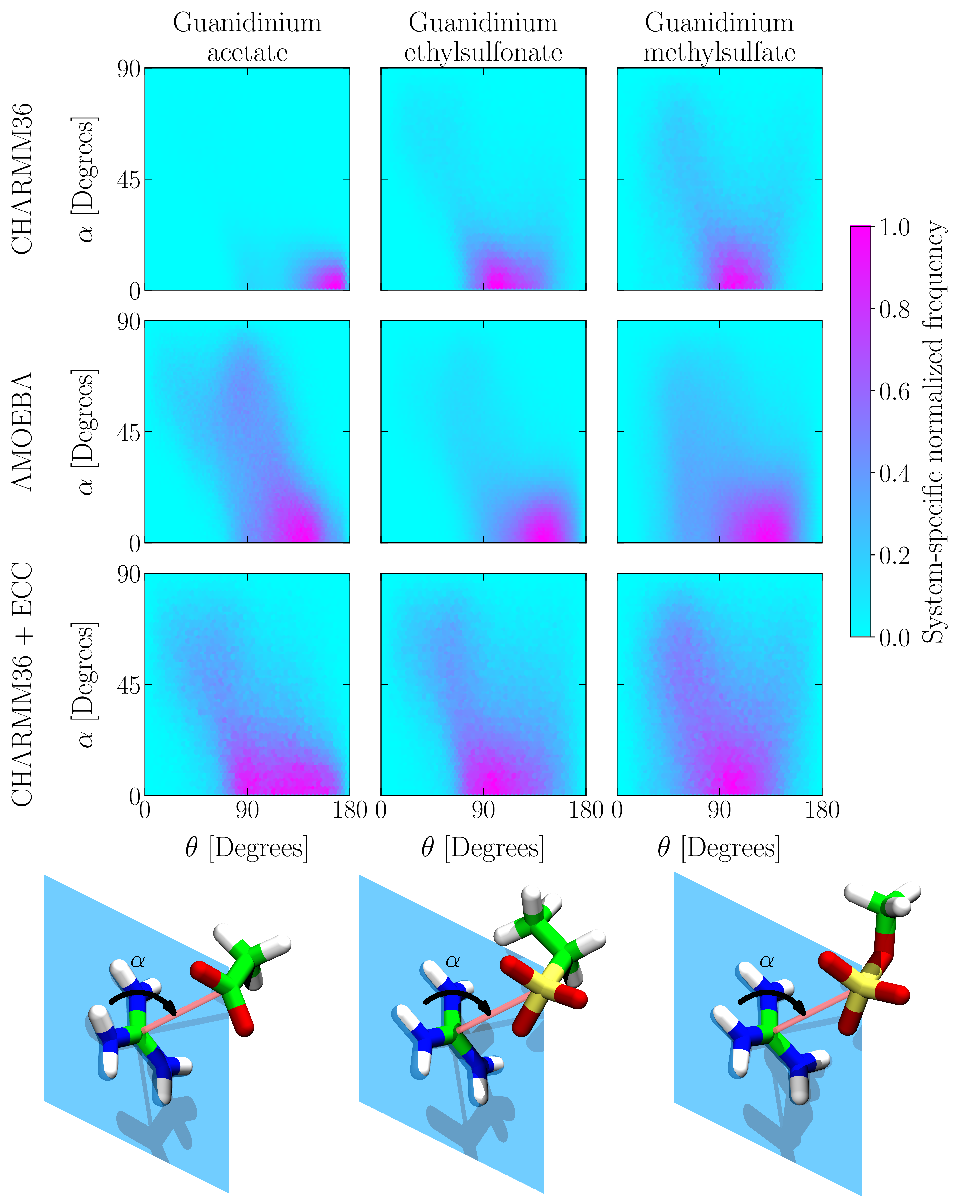
\includegraphics[width=\textwidth]{images/fig_hexmaps_guan.pdf}
        \caption{Heat maps of the sampling frequency of anion-guanidinium pairs (columns) with $r < R_{Shell}$ as observed in simulations using different force fields (rows). The normalization of sampling frequency is specific to each system. Refer to Table~\ref{tab:coordinates} for the definitions of $\theta$ and $\alpha$.}
        \label{fig:heatmap_guan}
    \end{center}
    \end{figure}
    
    \begin{figure}[H]
    \begin{center}
        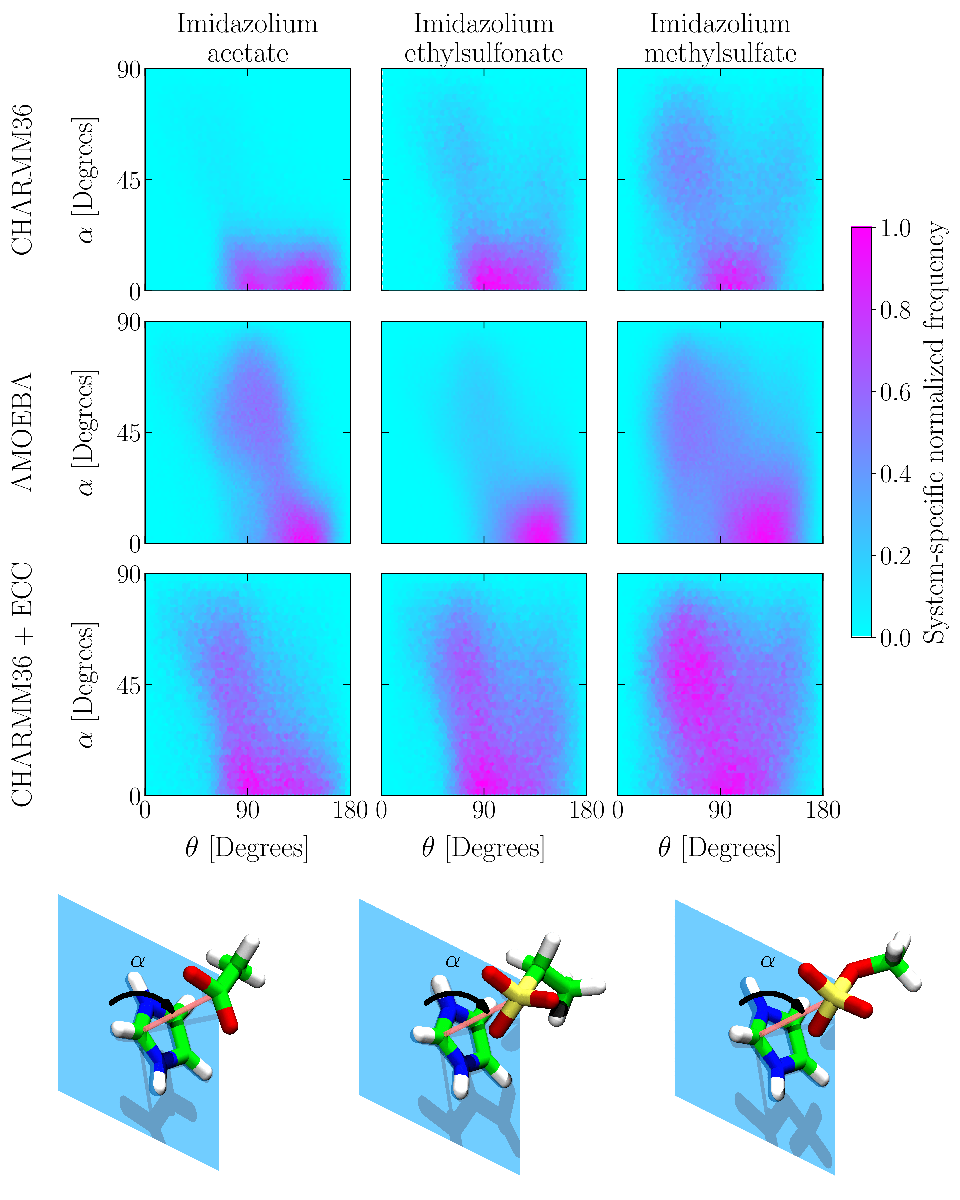
\includegraphics[width=\columnwidth]{images/fig_hexmaps_imim.pdf}
        \caption{Heat maps of the sampling frequency of anion-imidazolium pairs (columns) with $r < R_{Shell}$ as observed in simulations using different force fields (rows). The normalization of sampling frequency is specific to each system. Refer to Table~\ref{tab:coordinates} for the definitions of $\theta$ and $\alpha$.}
        \label{fig:heatmap_imim}
    \end{center}
    \end{figure}

    \begin{figure}[H]
    \begin{center}
        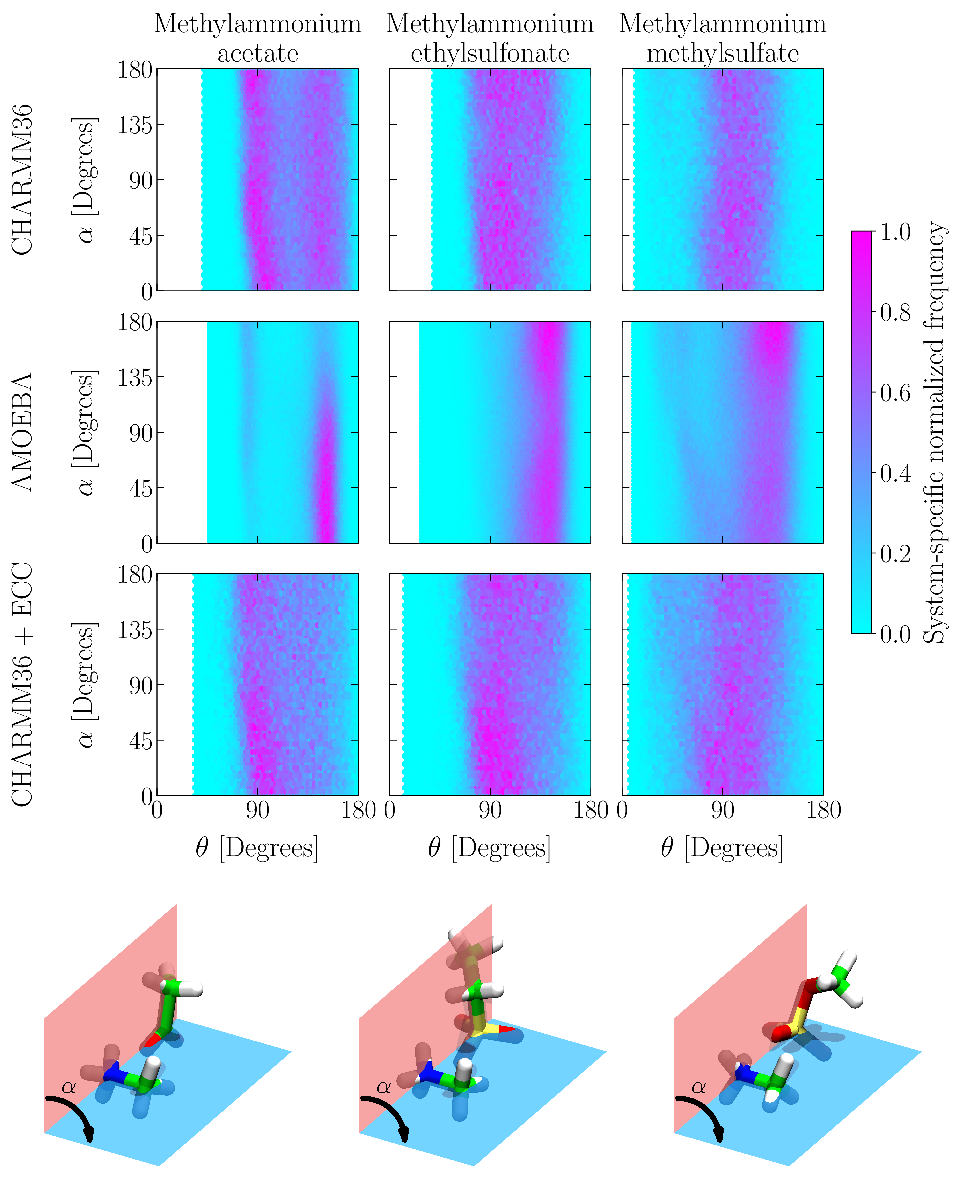
\includegraphics[width=\columnwidth]{images/fig_hexmaps_mamm.pdf}
        \caption{Heat maps of the sampling frequency of anion-methylammonium pairs (columns) with $r < R_{Shell}$ as observed in simulations using different force fields (rows). The normalization of sampling frequency is specific to each system. Refer to Table~\ref{tab:coordinates} for the definitions of $\theta$ and $\alpha$.}
        \label{fig:heatmap_mamm}
    \end{center}
    \end{figure}





    \section{Hydration free energy ($\mu^{\rm{ex}}$) simulations}
    \subsection{Molecular quasichemical theory (mQCT) and methods}

    The hydration free energy of a solute is formally defined by the solute's excess chemical potential $\mu^{\rm{ex}}$, which represents the contribution of the solute's intermolecular interactions in solution to the system Gibbs free energy. According to the potential distribution theorem \cite{Beck2006}
    \begin{eqnarray}
    \beta \mu^{\rm{ex}} = \ln \int e^{\beta \varepsilon} P(\varepsilon) d\varepsilon = \ln \langle e^{\beta \varepsilon} \rangle
    \label{eq:pdt}
    \end{eqnarray}
    where $\beta = 1/k_{\rm B}T$, $k_{\rm B}$ is Boltzmann's constant, $T$ is temperature, $\varepsilon$ is the solute-solvent interaction energy and $P(\varepsilon)$ is the probability density distribution of $\varepsilon$. To make $\mu^{\rm{ex}}$ amenable to estimation from molecular simulation, Equation \ref{eq:pdt} may be partitioned according to molecular quasichemical theory as \cite{Asthagiri2021b, Weber2012, Tomar2016, Adhikari2022, Weber2011}
    \begin{eqnarray}
    \beta \mu^{\rm{ex}} = \underbrace{- \ln p_0[\phi(r; \lambda_G)]}_\text{Packing} + \underbrace{\beta\mu^{\rm{ex}}_{\rm{LR}}[P(\varepsilon \; | \; \phi(r; \lambda_G))]}_\text{Long-range} + \underbrace{\ln x_0[\phi(r; \lambda_G)]}_\text{Chemistry}
    \label{eq:qct}
    \end{eqnarray}
    where $- \ln p_0$ represents packing (primitive hydrophobic) contributions to $\mu^{\rm{ex}}$, which corresponds to the free energy required to open a cavity in the liquid that can accommodate the solute. Long-range solute-solvent interaction energy contributions are represented by $\mu^{\rm{ex}}_{\rm{LR}}$ and $\ln x_0$ refers to the contribution of short-range chemical interactions that occur in the solute's inner hydration shell. Each of these terms are functionals of an imposed potential field $\phi$ that is used to move the solvent interface a distance $\lambda$ away from the solute but the sum of these terms is in principle independent of $\phi$. The probability distribution $P(\varepsilon|\phi)$ is that of $\varepsilon$ when the solvent is conditioned by $\phi$. In this work the soft repulsive WCA potential is used to define $\phi$ as \cite{Tomar2016, Adhikari2022, Weber2012}
    \begin{eqnarray}
    \phi (r_{ij} ; \lambda) = 
    \begin{cases}
        4a \left( \left( \dfrac{b}{r_{ij} - \lambda +  \sqrt[6]{2}b} \right)^{12} - \left( \dfrac{b}{r_{ij} - \lambda +  \sqrt[6]{2}b} \right)^{6} \right) + a, &  r_{ij} < \lambda \\
        0, & r_{ij} \ge \lambda
    \end{cases}
    \label{eq:wca_potential}
    \end{eqnarray}
    with parameters $a = 0.155$~kcal/mol and $b = 3.1655$~\AA\ selected from the SPC/E water model.\cite{Berendsen1987, Chatterjee2008} Here $r_{ij}$ represents the distance between solvent atom $i$ and solute atom $j$; in practice the potential is applied only to the water oxygen atoms based on the position of the solute heavy atoms. The union of spherical shells of radius $\lambda$ that are centered on the solute heavy atoms therefore defines the solute envelope and $\lambda$ may be understood as the range of $\phi$. The upper range is chosen to evacuate the inner hydration shell around the solute of interest such that $P(\varepsilon|\phi)$ may be described using a Gaussian distribution; this upper range is denoted $\lambda_G$ and was taken to be 5 \AA\ based on previous reports. \cite{Asthagiri2017, Adhikari2022}

    The magnitude of the WCA repulsive force is given by
    \begin{eqnarray}
    F(r_{ij} ; \lambda) = -\frac{\partial \phi}{\partial r_{ij}} = 
    \begin{cases}
         \dfrac{-24 a}{b} \left( \dfrac{b}{r_{ij} - \lambda +  \sqrt[6]{2}b} \right)^7 \left(1-2 \left( \dfrac{b}{r_{ij} - \lambda +  \sqrt[6]{2}b} \right)^6 \right), &  r_{ij} < \lambda \\
        0, & r_{ij} \ge \lambda
    \end{cases}
    \label{eq:wca_force}
    \end{eqnarray}
    and the total force exerted by the solvent on the solute-solvent interface at $\lambda$ may be obtained in practice as 
    \begin{eqnarray}
    F_{\rm{Wall}}(\lambda) = \sum_{i=1}^{N_{\rm{Solvent}}} \sum_{j=1}^{N_{\rm{Centers}}} F(r_{ij} ; \lambda)
    \label{eq:fwall}
    \end{eqnarray}
    where the summations in $i$ and $j$ proceed over the number of solvent molecules and the number of heavy atom centers in the solute, respectively. Packing contributions to $\mu^{\rm{ex}}$ are computed as 
    \begin{eqnarray}
    - \ln p_0[\phi(r; \lambda_G)] = \beta \int_{0}^{\lambda_G} \langle F_{\rm{Wall}} (\lambda) \rangle_{0} \; d \lambda
    \label{eq:packing}
    \end{eqnarray}   
    where $\langle F_{\rm{Wall}} (\lambda) \rangle_{0}$ is evaluated in the absence of the solute (i.e., with an uncoupled system) but the solvent is nonetheless conditioned by $\phi$ using fixed representative positions of the solute heavy atoms. Chemistry contributions may be similarly obtained as 
    \begin{eqnarray}
    \ln x_0[\phi(r; \lambda_G)] = -\beta \int_{0}^{\lambda_G} \langle F_{\rm{Wall}} (\lambda) \rangle \; d \lambda
    \label{eq:chemistry}
    \end{eqnarray}   
    where $\langle F_{\rm{Wall}} (\lambda) \rangle$ is evaluated in the presence of the solute (i.e. with a coupled system). In practice this integral may be evaluated over a smaller domain
    \begin{align}
    \ln x_0[\phi(r; \lambda_G)] &= -\beta \left( \int_{0}^{2 \; \text{\AA}} \langle F_{\rm{Wall}} (\lambda) \rangle \; d \lambda + \int_{2 \; \text{\AA}}^{\lambda_G} \langle F_{\rm{Wall}} (\lambda) \rangle \; d \lambda \right) \\
    &\approx -\beta \int_{2 \; \text{\AA}}^{\lambda_G} \langle F_{\rm{Wall}} (\lambda) \rangle \; d \lambda
    \label{eq:chemistry_2A}
    \end{align}
    because it is known from past experience that solvent never enters the domain of $\lambda~<~2.5~\text{\AA}$ when the solute is present \cite{Tomar2016}; integral contributions up to 2~\AA\ are therefore recognized as negligible. Assuming that $\lambda_G$ is sufficiently large to describe $P(\varepsilon|\phi)$ as a Gaussian, the long-range contributions may be obtained from a linear response model as \cite{Tomar2016, Adhikari2022}
    \begin{eqnarray}
    \beta \mu^{\rm{ex}}_{\rm{LR}}[P(\varepsilon \; | \; \phi(r; \lambda_G))] = \beta \langle \varepsilon \rangle_{\phi(\lambda_G)} + \beta^2 \frac{\sigma_{\phi(\lambda_G)}^2}{2}
    \label{eq:long-range}
    \end{eqnarray}
    where $\langle \varepsilon \rangle_{\phi(\lambda_G)}$ and $\sigma_{\phi(\lambda_G)}^2$ represent the mean and variance  of $P(\varepsilon|\phi)$, respectively, which is evaluated in the presence of the solute (i.e., with a coupled system) with $\phi(\lambda_G)$. 

    Equations \ref{eq:packing} and \ref{eq:chemistry_2A} were evaluated using 7-point Gauss–Legendre quadrature \cite{Hummer1996a} over each unit \AA\ such that 35 and 21 points were used in total, respectively, given that $\lambda_G~=~5~\text{\AA}$. Simulations were performed in sequence of increasing $\lambda$ with one ionic solute held in fixed position at the center of a box containing 1500 water molecules (box length $\sim$ 35.6 \AA), and the last configuration of one simulation was used as the starting configuration for the next $\lambda$ point. The Tcl-interface to NAMD and the \texttt{CustomExternalForce} class in OpenMM were used to impose $\phi$ in classical and semiclassical simulations, respectively. Classical simulations of 1~ns were performed at each $\lambda$ point with force data output saved every 50~fs and the last 0.5~ns of data were used for estimation of the mean $F_{\rm{Wall}} (\lambda)$. Analogous semiclassical simulations were run for 0.4~ns with data output every 25~fs and the last 0.3~ns were used for analysis. The standard error of the mean force was estimated using the Friedberg-Cameron algorithm\cite{Friedberg1970, Allen1986} and errors were propagated during integration using standard variance addition rules.
    
    For the evaluation of Equation \ref{eq:long-range} both classical and semiclassical simulations were performed for 1~ns with coordinates saved every 100~fs and the last 0.9~ns of data were used for analysis. As in the \emph{in vacuo} energy analyses, the \texttt{pairInteraction} module in NAMD was used to extract directly the net solute-solvent interaction energy from classical simulation frames. Separate \texttt{.arc} files were generated from semiclassical simulation trajectories for the solute + solvent system as well as the collection of solvent molecules. These were analyzed using the Tinker potential energy program \texttt{analyze} to obtain the total intermolecular interaction energy of the solute + solvent system $U_{N+1}$ as well as the interaction energy among all solvent molecules $U_{N}$, and the solute-solvent interaction energy was obtained as $U_{N+1} - U_{N}$.

    Ewald self-interaction corrections were computed following Hummer et al. and added to $\mu^{\rm{ex}}_{\rm{LR}}$.\cite{Hummer1996} CHARMM36 partial charge distributions were used in estimating Ewald corrections for both classical and semiclassical simulations. We note that these corrections apply to long-range interactions that are not sensitive to the details of the charge distribution (values are given in Table~\ref{tab:mqct_results} and are $-13.18 \pm 0.04$ kcal/mol for all ions in classical simulations) and errors arising from this approximation for semiclassical simulations are expected to be less than the uncertainty in the total $\mu^{\rm{ex}}_{\rm{LR}}$ estimate.

    To validate the applicability of the linear response model (Equation \ref{eq:long-range}), the distribution of interaction energy between the solute and conditioned solvent $P(\varepsilon | \phi(\lambda_G))$ was plotted for each system in Figure~\ref{fig:gaussian_check} alongside its best-fit Gaussian curve. To a good approximation $P(\varepsilon | \phi(\lambda_G))$ is observed to conform to the Gaussian expectation. However, as an orthogonal check, long-range contributions were also computed more rigorously in CHARMM36 using an alchemical transformation to estimate the electrostatic contributions, which are the primary determinant of the final $\mu^{\rm{ex}}_{\rm{LR}}$ value in the absence of polarization. The less substantial van der Waals contributions were still computed using a linear response model, so $\mu^{\rm{ex}}_{\rm{LR}}$ was obtained as
    \begin{equation}
    \beta \mu^{\rm{ex}}_{\rm{LR}}[P(\varepsilon \; | \; \phi(r; \lambda_G))] = \beta \langle \varepsilon \rangle_{\rm{Vdw}, \phi(\lambda_G)} + \beta^2 \frac{\sigma_{\rm{Vdw}, \phi(\lambda_G)}^2}{2} + \beta \int_{0}^{1} \biggl< \sum_{n=1}^{N_{Atoms}} q_n \psi_n (\gamma q_n) \biggr>_{\phi(\lambda_G)} d \gamma
    \label{eq:charging_validation}
    \end{equation}
    where the sum is over all solute atoms, the coupling parameter $\gamma$ scales the atomic partial charges $q_n$ and the electrostatic potential at each solute atom $\psi_n$ is evaluated for scaled partial charges $\gamma q_n$. The values of $\langle \varepsilon \rangle_{\rm{Vdw}, \phi(\lambda_G)}$ and $\sigma_{\rm{Vdw}, \phi(\lambda_G)}$ were estimated using a simulation in which $q_n = 0 \; \forall \; n$. Simulations of 1~ns were performed at 3 Gauss–Legendre quadrature points in $\gamma$ to estimate the integral in Equation \ref{eq:charging_validation}; coordinates were saved every 200~fs and the last 0.8~ns of data were used for analysis. The results are juxtaposed with the linear-response model estimates of $\mu^{\rm{ex}}_{\rm{LR}}$ in Figure~\ref{fig:long_range_method_parity}, showing that the error incurred by using a linear-response model in the reported results is on the order of only a few percent of the $\mu^{\rm{ex}}_{\rm{LR}}$ value.






    \pagebreak
    \begin{landscape}
    \subsection{Supplementary mQCT results}

    \begin{adjustbox}{center, addcode={%
        \begin{minipage}{\width}
        }{
        \caption[Short Caption]{mQCT contributions to ion hydration free energies. All values are in kcal/mol and uncertainties represent the standard error of the mean.}\label{tab:mqct_results}
        \end{minipage}
        }, float=table
        }
    % \begin{adjustbox}{center, caption={mQCT contributions to ion hydration free energies. All values are in kcal/mol and uncertainties represent the standard error of the mean.}, float=table}
    % \label{tab:mqct_results}
    \centering
    \renewcommand{\arraystretch}{0.7}
    \begin{tabular}{c | c | c | c | c | c | c | c } % llllllll
    Force field & Ion & Packing & Uncorrected & Ewald & Corrected & Chemistry & Total \\
     & & & long-range & correction & long-range & & \\ \hline
    CHARMM36    & Acetate        & $22.03 \pm 0.08$ & $-39.86 \pm 0.11$ & $-13.22$ & $-53.08 \pm 0.11$ & $-65.79 \pm 0.08$ & $-96.84 \pm 0.16$ \\
    CHARMM36    & Ethylsulfonate & $27.09 \pm 0.12$ & $-38.68 \pm 0.10$ & $-13.20$ & $-51.87 \pm 0.10$ & $-57.76 \pm 0.08$ & $-82.54 \pm 0.18$ \\
    CHARMM36    & Methylsulfate  & $26.41 \pm 0.11$ & $-35.83 \pm 0.10$ & $-13.16$ & $-48.99 \pm 0.10$ & $-53.37 \pm 0.10$ & $-75.96 \pm 0.18$ \\
    CHARMM36    & Guanidinium    & $21.91 \pm 0.09$ & $-19.99 \pm 0.09$ & $-13.14$ & $-33.13 \pm 0.09$ & $-47.89 \pm 0.08$ & $-59.11 \pm 0.15$ \\
    CHARMM36    & Imidazolium    & $22.32 \pm 0.08$ & $-19.90 \pm 0.09$ & $-13.15$ & $-33.05 \pm 0.09$ & $-37.23 \pm 0.07$ & $-47.96 \pm 0.14$ \\
    CHARMM36    & Methylammonium & $17.57 \pm 0.07$ & $-23.17 \pm 0.09$ & $-13.22$ & $-36.38 \pm 0.09$ & $-39.00 \pm 0.06$ & $-57.82 \pm 0.13$ \\ \hline
    AMOEBA      & Acetate        & $23.92 \pm 0.28$ & $-29.20 \pm 0.19$ & $-13.19$ & $-42.39 \pm 0.19$ & $-67.17 \pm 0.24$ & $-85.64 \pm 0.42$ \\
    AMOEBA      & Ethylsulfonate & $29.76 \pm 0.28$ & $-27.16 \pm 0.21$ & $-13.16$ & $-40.31 \pm 0.21$ & $-58.00 \pm 0.29$ & $-68.55 \pm 0.45$ \\
    AMOEBA      & Methylsulfate  & $29.59 \pm 0.30$ & $-28.60 \pm 0.20$ & $-13.14$ & $-41.74 \pm 0.20$ & $-54.46 \pm 0.23$ & $-66.61 \pm 0.43$ \\
    AMOEBA      & Guanidinium    & $23.29 \pm 0.33$ & $-28.81 \pm 0.13$ & $-13.11$ & $-41.92 \pm 0.13$ & $-43.13 \pm 0.22$ & $-61.76 \pm 0.41$ \\
    AMOEBA      & Imidazolium    & $24.33 \pm 0.25$ & $-28.77 \pm 0.14$ & $-13.12$ & $-41.90 \pm 0.14$ & $-39.18 \pm 0.22$ & $-56.75 \pm 0.36$ \\
    AMOEBA      & Methylammonium & $18.51 \pm 0.29$ & $-32.23 \pm 0.15$ & $-13.19$ & $-45.42 \pm 0.15$ & $-45.31 \pm 0.28$ & $-72.22 \pm 0.43$
    \end{tabular}
    \end{adjustbox}
    \end{landscape}

    \begin{figure}[H]
    \begin{center}
        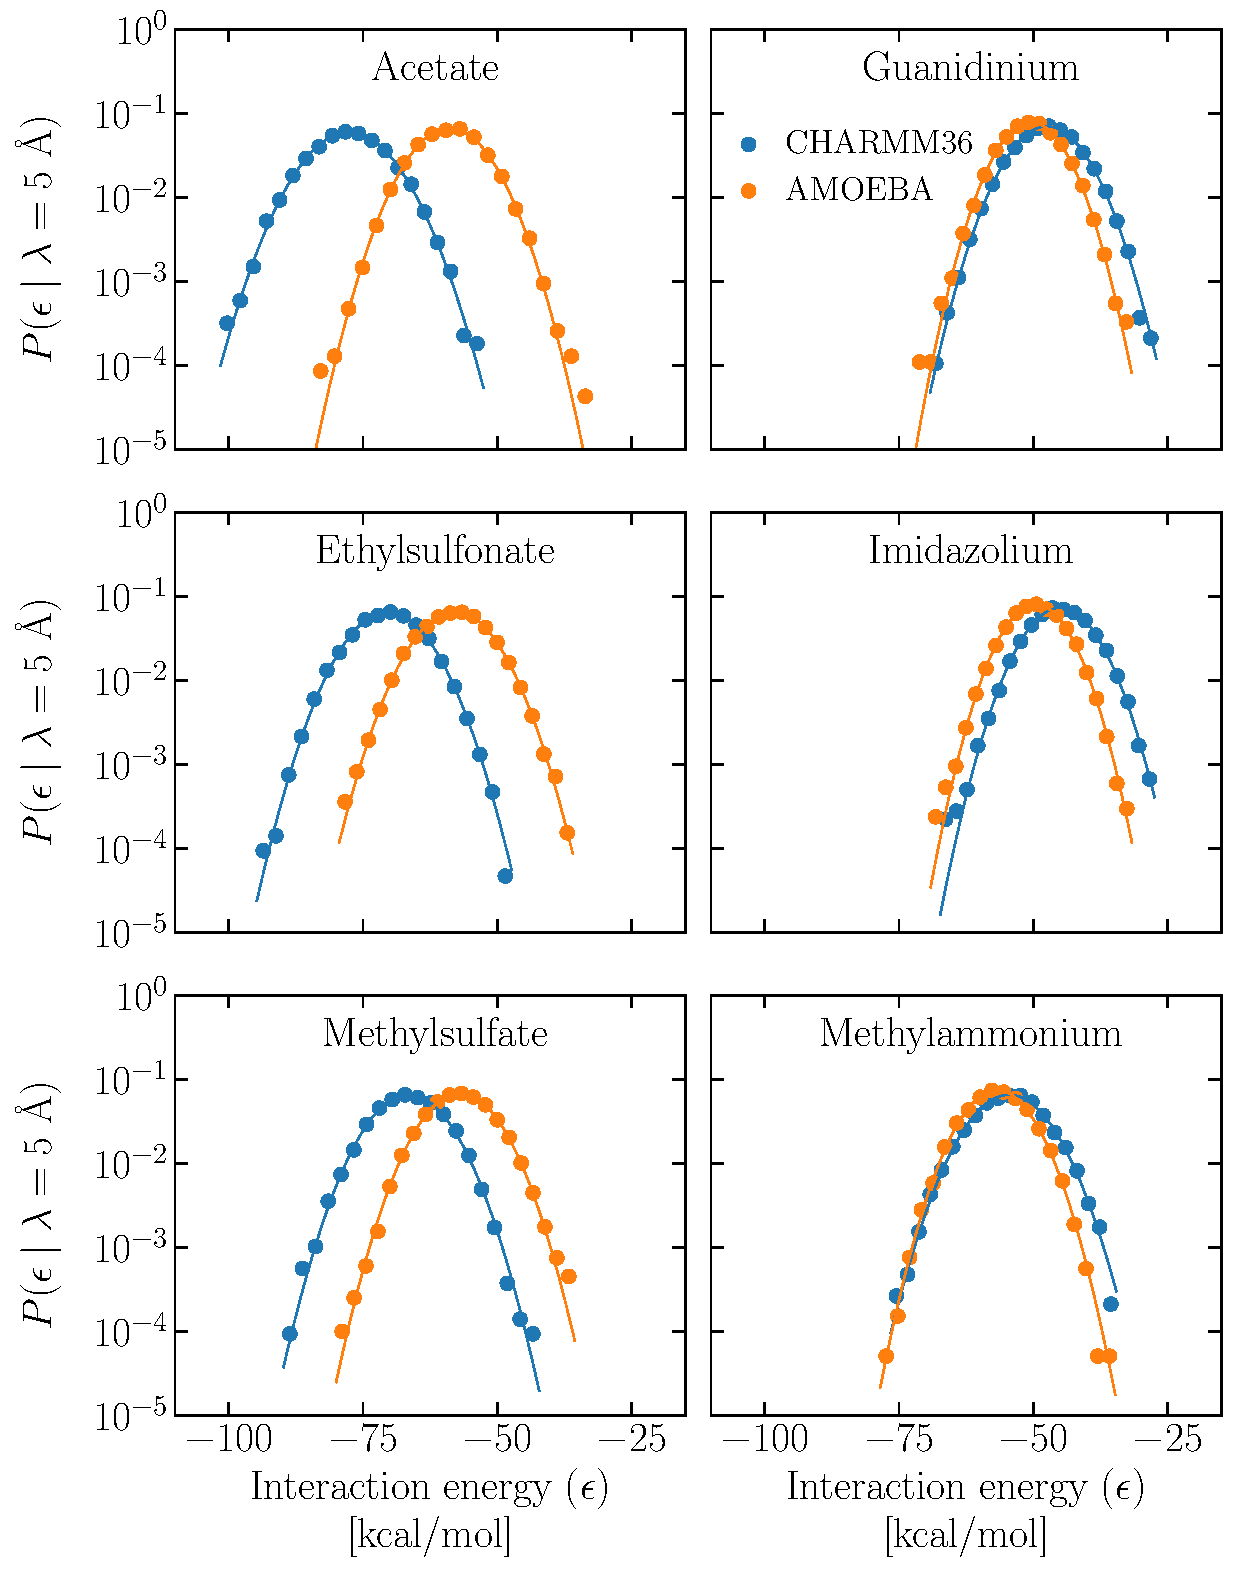
\includegraphics[width=0.95\columnwidth]{images/gaussian_check.pdf}
        \caption{Interaction energy distributions between ions and the solvent when conditioned by $\phi(\lambda_G)$. Points represent the simulation data and lines represent Gaussian fits with the same mean and standard deviation as the data.}
        \label{fig:gaussian_check}
    \end{center}
    \end{figure}
    
    \begin{figure}[H]
    \begin{center}
        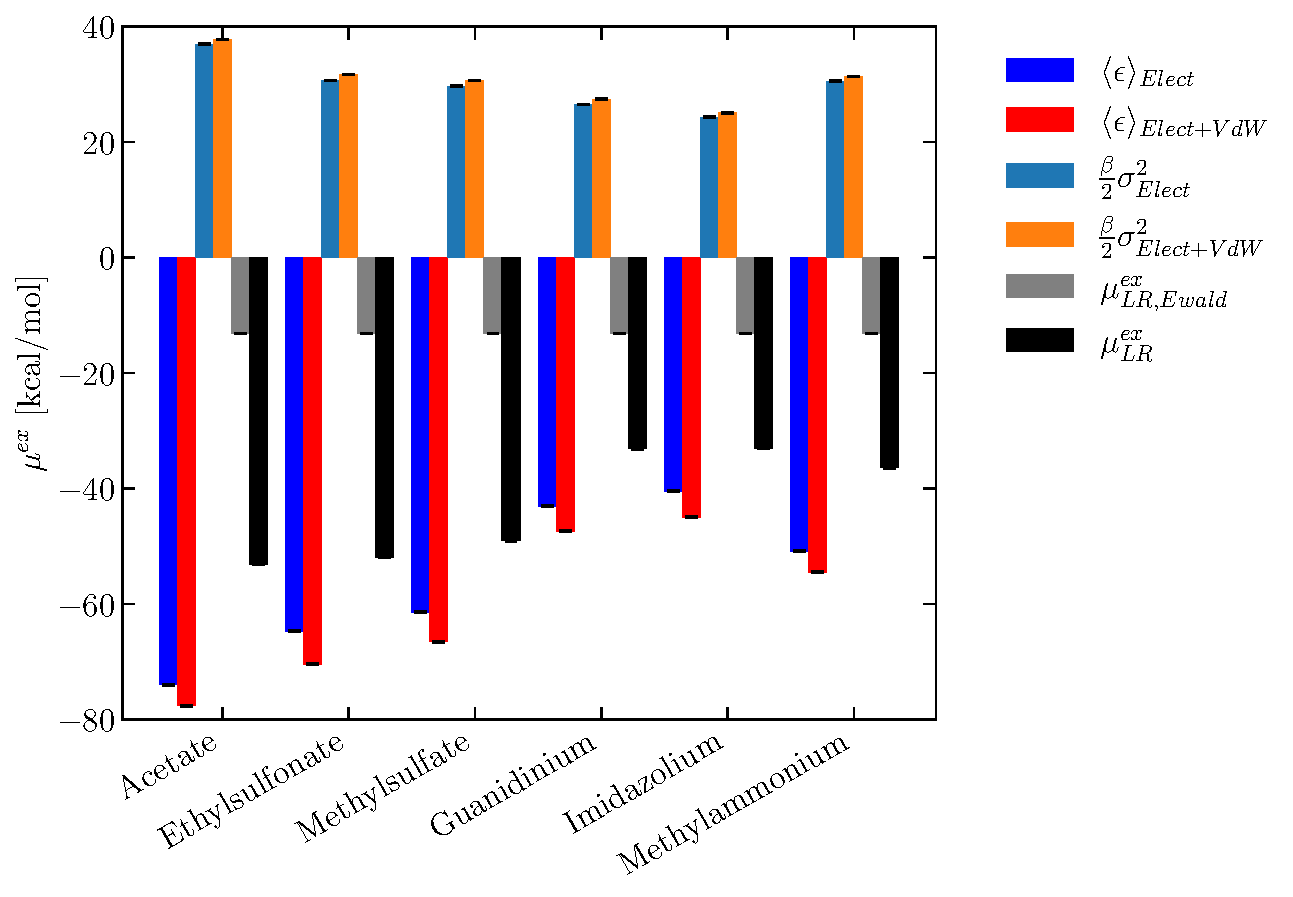
\includegraphics[width=0.49\columnwidth]{CEX/images/long_range_charmm.pdf}
        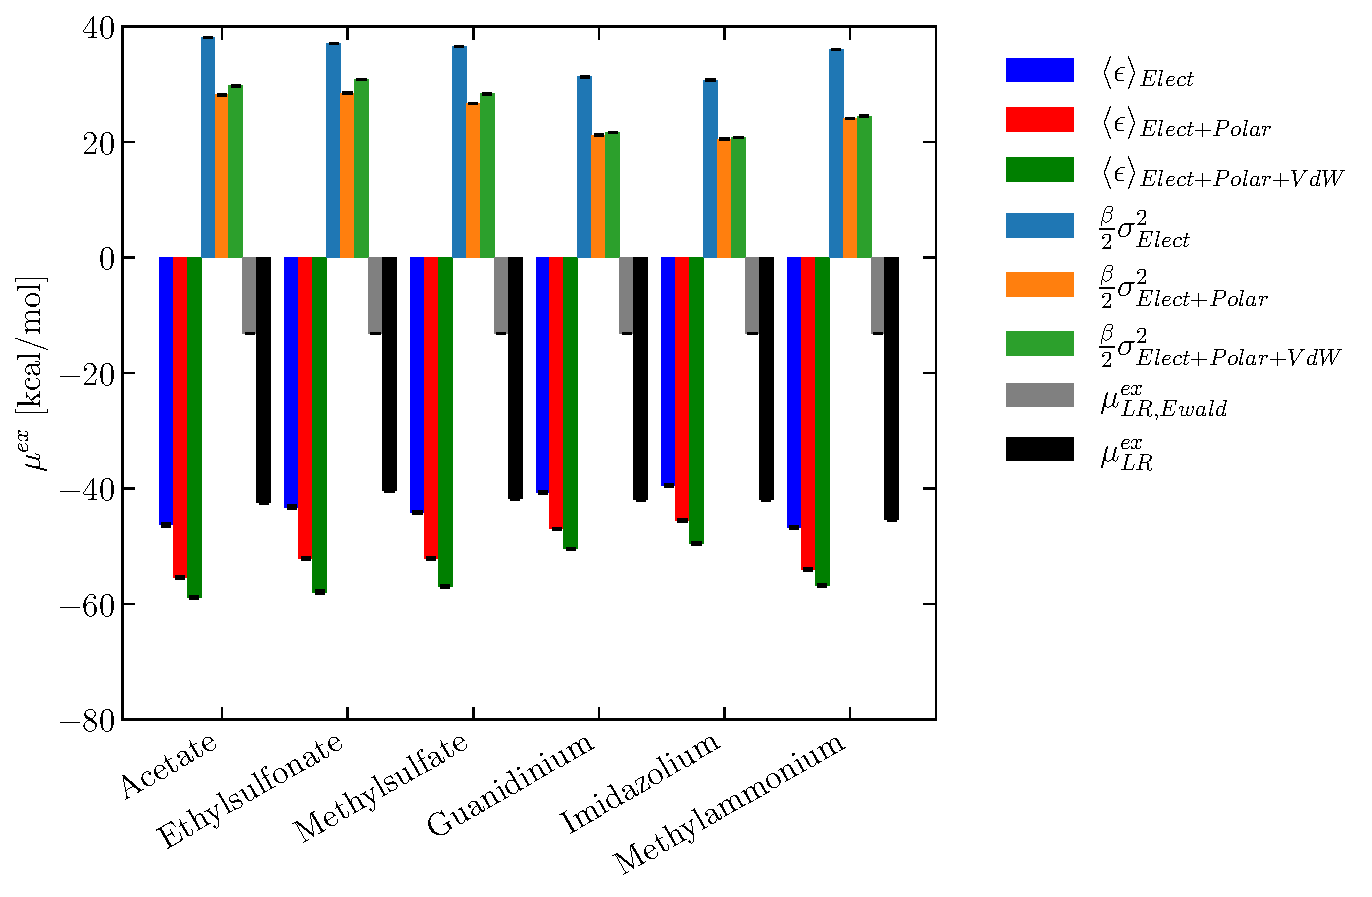
\includegraphics[width=0.49\columnwidth]{CEX/images/long_range_amoeba.pdf}
        \caption{Comparison of the components of long-range contributions to the hydration free energy for CHARMM36 and AMOEBA. Error bars represent $2\times$ the standard error of the mean. The results show that multipole electrostatics itself reduces the difference between long-range components of anions and cations. }
        \label{fig:long_range_compare}
    \end{center}
    \end{figure}
    
    \begin{figure}[H]
    \begin{center}
        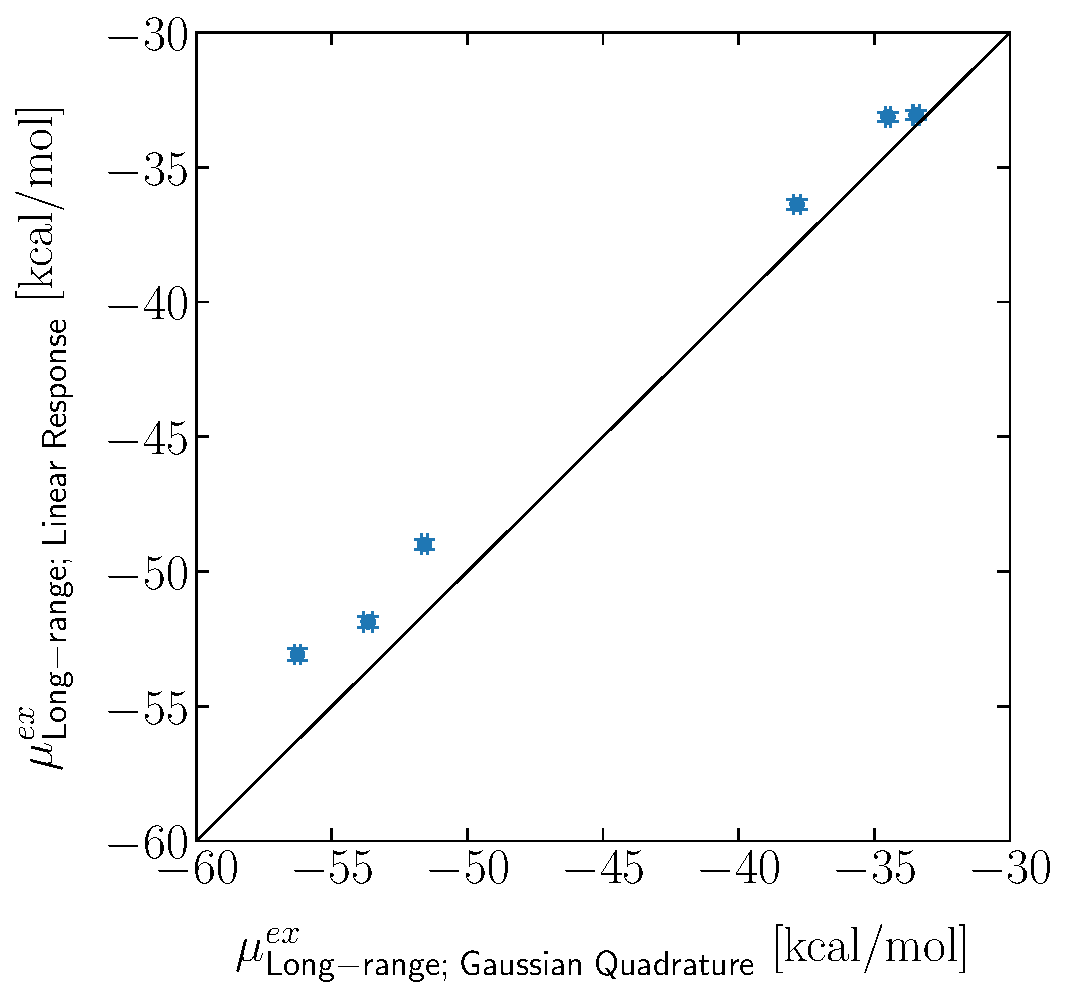
\includegraphics[width=0.7\columnwidth]{images/long_range_method_parity.pdf}
        \caption{Comparison of Ewald-corrected long-range contributions to the hydration free energy as estimated in CHARMM36 using either 3-point Gaussian quadrature for electrostatic contributions (abscissa, Equation \ref{eq:charging_validation}) or the linear response model (ordinate, Equation \ref{eq:long-range}). Error bars represent $2\times$ the standard error of the mean.}
        \label{fig:long_range_method_parity}
    \end{center}
    \end{figure}




    \clearpage
    \section{Estimation of $\mu^{\rm{ex}}$ from experimental data}
    
    \subsection{Thermodynamic cycle}
    
    \begin{figure}[H]
    \begin{center}
        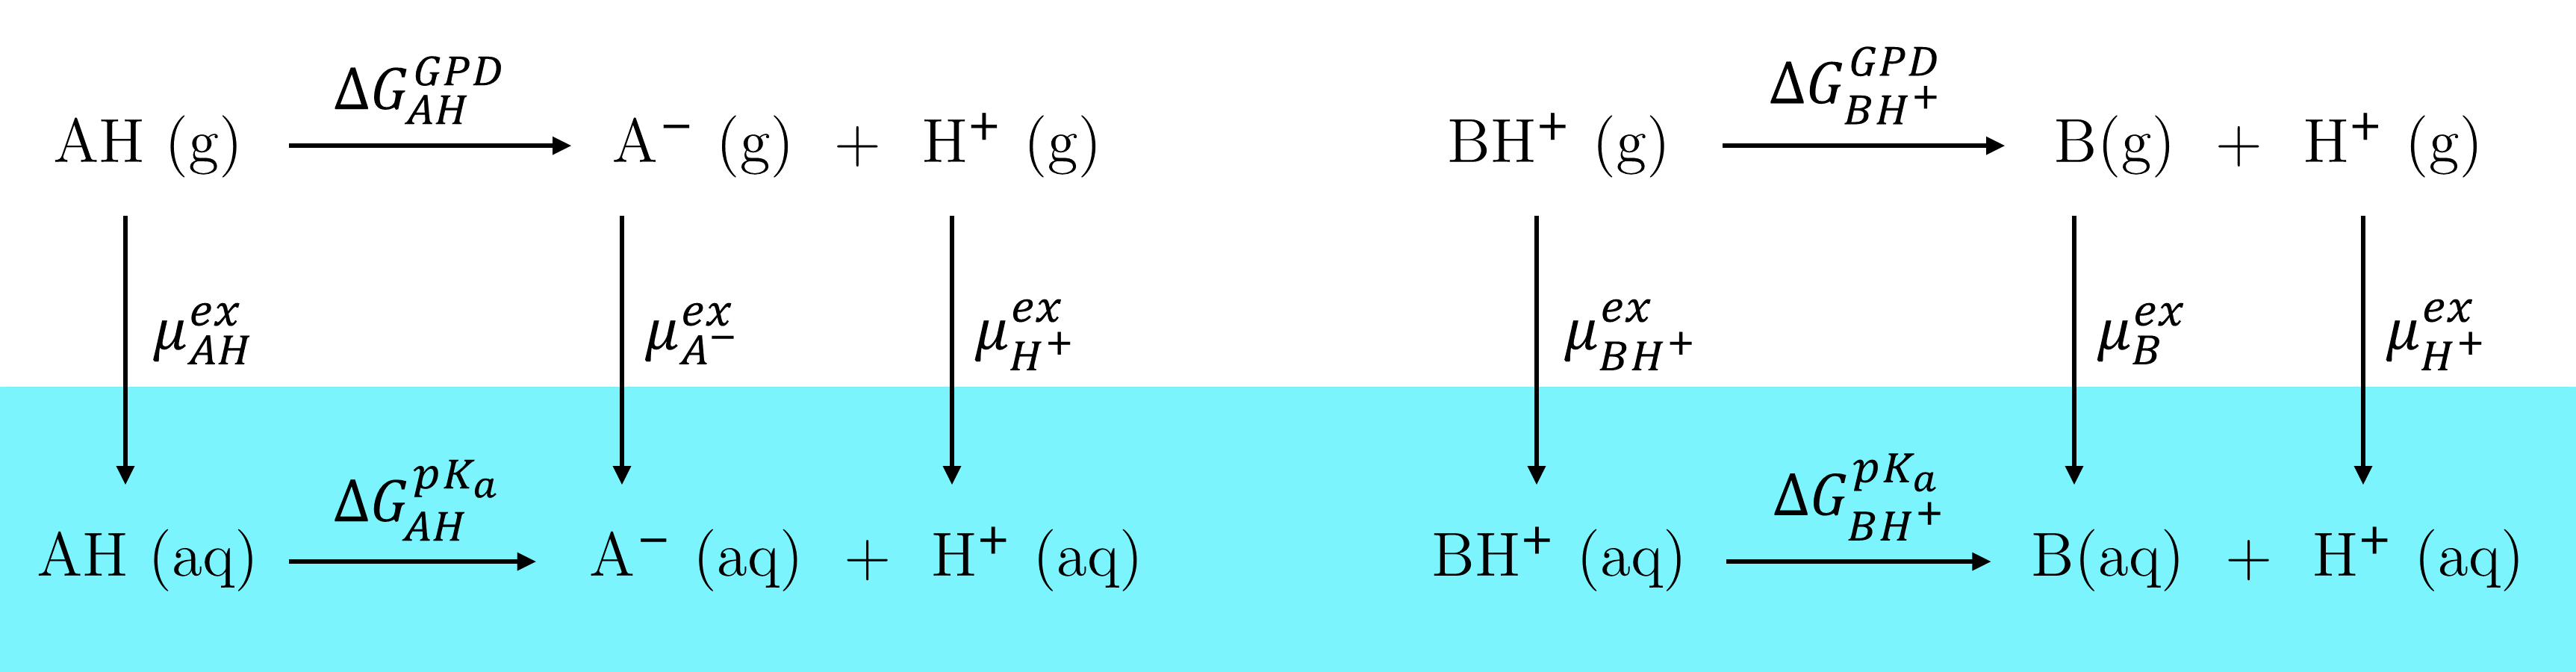
\includegraphics[width=1\columnwidth]{images/thermo_cycle_v1.png}
        \caption{Thermodynamic cycles that were used to estimate anion ($\ce{A^-}$, left) and cation ($\ce{BH^+}$, right) hydration free energies from experimental data.}
        \label{fig:thermo_cycle}
    \end{center}
    \end{figure}
    
    We have used thermodynamic cycles based on proton dissociation (TCPD, Figure~\ref{fig:thermo_cycle})\cite{Fossat2021, Lim1991, Pearson1986} to estimate $\mu^{\rm{ex}}$ from experimental data for comparison with simulation results. Specifically, $\mu^{\rm{ex}}$ was estimated for anions ($\ce{A^-}$) and cations ($\ce{BH^+}$) as
    \begin{equation}
    \mu^{\rm{ex}}_{A^-} = \mu^{\rm{ex}}_{AH} - \Delta G^{\rm{GPD}}_{AH} + \Delta G^{pK_a}_{AH} - \mu^{\rm{ex}}_{H^+} 
    \label{eq:tcpd_anion}
    \end{equation}
    \begin{equation}
    \mu^{\rm{ex}}_{BH^+} = \mu^{\rm{ex}}_{B} + \Delta G^{\rm{GPD}}_{BH^+} - \Delta G^{pK_a}_{BH^+} + \mu^{\rm{ex}}_{H^+} 
    \label{eq:tcpd_cation}
    \end{equation}
    where $\mu^{\rm{ex}}_{AH \; / \; B}$ represents the hydration free energy of the corresponding neutral conjugate $\ce{AH}$ or $\ce{B}$, $\Delta G^{\rm{GPD}}_{AH \; / \; BH^+}$ represents the free energy change of the gas-phase deprotonation of $\ce{AH}$ or $\ce{BH^+}$ (i.e., the gas-phase basicity of the cation conjugate base $\ce{B}$), $\Delta G^{pK_a}_{AH \; / \; BH^+}~=~2.30~RT~pK_a$ represents the corresponding free energy change of titration in the aqueous phase and $\mu^{\rm{ex}}_{H^+}$ represents the proton hydration free energy. In this work $\mu^{\rm{ex}}_{H^+}$ was taken to be $-260.9~\pm~5.8$ kcal/mol, which represents the mean and standard deviation of 72 independent estimates.\cite{Fossat2021} The appreciable uncertainty that surrounds this value is due to the extrathermodynamic assumptions that must be made to deconvolute measurable salt hydration free energies into anion and cation contributions, which are not directly accessible to experiment.\cite{Grossfield2003} Experimental uncertainties were not reported for much of the required data, so a representative uncertainty of 2.5 kcal/mol was assumed for the sum of the first three terms on the right-hand side of equations \ref{eq:tcpd_anion} and \ref{eq:tcpd_cation}, leading to a total uncertainty of 6.3 kcal/mol in the $\mu^{\rm{ex}}$ estimates for anions and cations. Although this is larger than what is typically reported by independent experimental studies, this uncertainty reflects the inherent ambiguities of estimating single ion hydration free energies and using the TCPD with a constant $\mu^{\rm{ex}}_{H^+}$ enables a consistent comparison with simulation results.




    \subsection{Experimental estimates of $\mu^{\rm{ex}}$}
    
    \begin{adjustbox}{center, 
    caption={Ions for which complete experimental data sets exist to estimate $\mu^{\rm{ex}}$ using a thermodynamic cycle based on proton dissociation (TCPD). \cite{Fossat2021, Lim1991, Pearson1986, Reif2012} TCPD estimates are based on a proton hydration free energy of $-260.9 \pm 5.8$ kcal/mol, which represents the mean and standard deviation of 72 independent estimates.\cite{Fossat2021} Experimental uncertainties were not reported for much of the required data, so a representative uncertainty of 2.5 kcal/mol was assumed for the sum of the first three terms on the right-hand side of equations \ref{eq:tcpd_anion} and \ref{eq:tcpd_cation}, leading to a total uncertainty of 6.3 kcal/mol in the $\mu^{\rm{ex}}$ estimates. $\mu^{\rm{ex}}_{AH \; / \; B}$ represents the hydration free energy of the neutral conjugate and $\Delta G^{\rm{GPD}}_{AH \; / \; BH^+}$ represents the free energy change of gas-phase deprotonation.}, float=table}
    \centering
    \label{tab:thermo_cycle_data}
    \renewcommand{\arraystretch}{0.8}
    \begin{threeparttable}
    \begin{tabular}{c | c | c | c | c | c}
    Ion & Neutral conjugate & $\mu^{\rm{ex}}_{AH \; / \; B}$ & $\Delta G^{\rm{GPD}}_{AH \; / \; BH^+}$ & $pK_a$ & TCPD estimate of \\
    (A$^-$ / BH$^+$) & (AH / B)  & [kcal/mol] & [kcal/mol] & & $\mu^{\rm{ex}}_{A^-}$ / $\mu^{\rm{ex}}_{BH^+}$ [kcal/mol] \\ \hline
    Acetate & Acetic acid & $-6.7$ \cite{Cramer1991} & $341.4 \pm 1.9$ \cite{Taft1987, Cumming1977, Fujio1981} & 4.76 \cite{Settimo2014} & $-80.7 \pm 6.3$\\
    Guanidinium & Guanidine & $-11.5$ \cite{Zhang2017}$^{,}$\tnote{a} & 226.9\cite{Hunter1998} & 13.65\cite{Wolfenden1981} & $-64.1 \pm 6.3$\\
    Imidazolium & Imidazole & $-9.63$ \cite{Rizzo2006} & 217.3 \cite{Hunter1998} & 7.05 \cite{Walba1961} & $-62.8 \pm 6.3$\\
    Methylammonium & Methylamine & $-4.56$ \cite{In2005} & 206.6 \cite{Hunter1998} & 10.6 \cite{Lim1991} & $-73.3 \pm 6.3$
    \end{tabular}
    \begin{tablenotes}
        \linespread{1}\small
        \item[a] This is an approximate experimental estimate based on the hydration free energy of methylguanidine ($-11.2$~kcal/mol)\cite{Wolfenden1981}, which was decreased by 0.3~kcal/mol in an attempt to remove the contribution of the methyl group.\cite{Reif2012} 
    \end{tablenotes}
    \end{threeparttable}
    \end{adjustbox}    

    \clearpage

    \begin{adjustbox}{center, 
    caption={Comparison of mQCT and experimental estimates of ion hydration free energies. All values are in kcal/mol. Uncertainties in mQCT results represent the standard error of the mean, whereas the reported uncertainties in experimental estimates represent the measurement standard deviation. Where available, the first entry in the list of experimental data represents the TCPD estimate and the subsequent entries were taken directly from the literature (without correction for any differences in free energy reference values that are related to the underlying extrathermodynamic assumptions).}, float=table}
    \centering
    \label{tab:mqct_lit_comparison}
    \renewcommand{\arraystretch}{0.8}
    \begin{threeparttable}
        \begin{tabular}{c | c | c | c }
        Ion            & CHARMM36 & AMOEBA & Experimental estimates \\ \hline
        Acetate        & $-96.84 \pm 0.16$ & $-85.64 \pm 0.42$ & $-80.7 \pm 6.3$,\tnote{a} \ \ $-75 \pm 2$ \cite{Pearson1986}, \ $-77$ \cite{Cramer1991}, \ $-79 \pm 3$ \cite{Gilson1988}, \ $-89.1$ \cite{Marcus2013} \\
        Ethylsulfonate & $-82.54 \pm 0.18$ & $-68.55 \pm 0.45$ & - \\
        Methylsulfate  & $-75.96 \pm 0.18$ & $-66.61 \pm 0.43$ & - \\
        Guanidinium    & $-59.11 \pm 0.15$ & $-61.76 \pm 0.41$ & $-64.1 \pm 6.3$,\tnote{a} \ \ $-139 \pm 2$ \cite{Marcus2012}$^{,}$\tnote{b} \\
        Imidazolium    & $-47.96 \pm 0.14$ & $-56.75 \pm 0.36$ & $-62.8 \pm 6.3$\tnote{a} \\
        Methylammonium & $-57.82 \pm 0.13$ & $-72.22 \pm 0.43$ & $-73.3 \pm 6.3$,\tnote{a} \ \ $-68 \pm 2$ \cite{Pearson1986}, \ $-70$ \cite{Cramer1991}, \ $-71\pm 3$ \cite{Gilson1988}    
        \end{tabular}
        \begin{tablenotes}
            \linespread{1}\small
            \item[a] Estimate based on the thermodynamic cycle (Table~S4).
            % Hard coded
            \item[b] Some controversy surrounds this measurement\cite{Houriez2017} and quantum mechanics estimates ($-57.9~\pm~0.8$ kcal/mol)\cite{Gokcen2014} are much closer to the values estimated using CHARMM36, AMOEBA and the thermodynamic cycle.            
        \end{tablenotes}
    \end{threeparttable}
    \end{adjustbox}






    
    \clearpage
    \bibliography{myref}
    
\end{document} 






